%versi 2 (8-10-2016)
\chapter{Landasan Teori}


\section{BlueTape}
Bluetape merupakan aplikasi berbasis web, berguna sebagai aplikasi yang menunjang proses administrasi dalam lingkungan FTIS UNPAR. Web ini dapat diakses pada \path{http://www.bluetape.azurewebsites.net}. \cite{blueTape}

\subsection{Login}
\label{ss:login}
Halaman utama aplikasi BlueTape akan mengarahkan \textit{user} untuk \textit{login} dengan menggunakan Google, user akan login dengan melihat beberapa kondisi ini:
\begin{itemize}
	\item Apabila \textit{user} belum pernah login menggunakan akun UNPAR(xxx@student.unpar.ac.id atau yyy@unpar.ac.id) maka  \textit{user} akan diminta untuk memasukan email UNPAR dan password
	\item Apabila user sudah pernah login menggunakan akun UNPAR, maka \textit{user} akan diminta untuk memilih akun beserta password.
	\item User akan terhubung otomatis dengan akun @gmail.com. Apabila BlueTape menolak autentikasi user maka: User akan diminta untuk buka halaman Gmail lalu klik avatar di kanan atas dan memilih akun UNPAR yang tepat pada tombol "Add Account"
\end{itemize}
User akan melihat beberapa menu sesuai dengan \textit{role} user, sebagai mahasiswa, staf TU, dll.

\subsection{Dosen}
\subsubsection{Perubahan Kuliah}
Modul perubahan kuliah berguna untuk mengirimkan permintaan perubahan mata kuliah yang dikirim oleh dosen kepada staf Tata Usaha. Kolom - kolom yang terdapat dalam modul ini:
\begin{itemize}
	\item Kode MK (Mata Kuliah)
	\item Nama Mata Kuliah
	\item Kelas
	\item Jenis perubahan (diganti / tambahan / ditiadakan)
	\item Dari (hari/jam dan ruang) dan ke(hari/jam dan tempat)
	\item Keterangan
\end{itemize}
Apabila ada kolom yang belum dapat diisi(contoh : dosen belum tahu tempat kelas pengganti) maka kolom kelas dapat dikosongkan.
Dosen juga dapat membuat lebih dari 1 kelas pengganti, dengan mengklik tombol "Tambah Pertemuan Ekstra".
Setelah dosen klik "Kirim Permohonan", maka sistem akan mengirim permohonan ke halaman BlueTape bagian Tata Usaha utnuk diperiksa, disetujui, dan dicetak sebagai pengumuman. Jika staf Tata Usaha telah selesai mengkonfirmasi(atau menolak), maka dosen akan mendapatkan e-mail notifikasi.

\subsection{Dosen Informatika}
\subsubsection{Entri Jadwal Dosen}
Dosen informatika dapat menggunakan menu ini untuk mengisikan jadwal mingguan. Hasil dari pengisian jadwal dapat diekspor ke XLS, atau dapat dilihat oleh mahasiswa informatika melalui portal BlueTape.
\subsubsection{Tambah Jadwal}
Pada bagian entri jadwal, dosen informatika dapat mengisikan hari, jam mulai, durasi, label, dan sejenisnya. Berikut ini jenis yang dapat dipilih:
\begin{itemize}
	\item Konsultasi : Waktu yang dosen siapkan untuk konsultasi mahasiswa. Pada tabel akan diberi \textit{background} berwaena kuning.
	\item Terjadwal: Kegiatan mingguan dosen informatika yang telah terjadwal. Contoh : rapat jurusan
	\item Kelas : Kelas kuliah maupun praktikum.
\end{itemize}
Lalu dosen dapat klik tombol "Tambah" untuk menambahkan

\subsubsection{Ubah/Hapus Jadwal}
Dosen dapat mengubah atau menghapus jadwal yang tertera pada tabel. Lalu \textit{pop-up} window akan terbuka dengan pilihan-pilihan yang sesuai dengan permintaan dosen.

\subsubsection{Hapus Semua}
Tombol "Delete All" dapat digunakan untuk menghapus secara cepat seluruh jadwal yang telah dosen buat sebelumnya. Penggunaan tombol ini biasa nya digunakan pada awal semester, dimana jadwal yang dosen miliki berubah seluruhnya.

\subsubsection{Ekspor ke XLS}
Tombol "Ekspor ke XLS" berfungsi untuk membuat file excel (.xls) untuk jadwal dosen.

\subsection{Mahasiswa}
\subsubsection{Cetak Transkrip}
Mahasiswa dapat menggunakan menu ini untuk mengirimkan permohonan cetak transkrip
Mahasiswa mengirimkan permohonan pencetakan transkrip dengan mengisi kolom-kolom pada formulir "Permohonan Baru".
Mahasiswa hanya dapat mengirimkan permohonan:
\begin{itemize}
	\item Maksimal 1x dalam satu semester (kecuali permohonan ditolak)
	\item Jika ada permohonan yang belum dijawab.
\end{itemize}

\subsubsection{Mahasiswa Informatika}
\subsubsection{Lihat Jadwal Dosen}
Mahasiswa dapat melihat jadwal mingguan seluruh dosen dengan memilih nama dosen pada seleksi tab, dan tabel jadwal dosen akan ditampilkan pada bagian bawah halaman. Selain itu tabel juga berisi informasi tanggal terakhir dosen meng-\textit{update} jadwal sehingga mahasiswa dapat melihat apakah jadwal tersebut merupakan jadwal semester ini atau semester lalu. 
Lalu terdapat tombol "Ekspor ke XLS" pada halaman lihat jadwal dosen, sehingga mahasiswa dapat menyimpan atau mencetak jadwal tersebut. 

\subsection{Staf Tata Usaha}
\subsubsection{Manajemen Perubahan Kuliah}
Staf Tata Usaha dapat melakukan manajemen permintaan perubahan kuliah. Sebuah tabel akan menampilkan daftar permohonan dengan menampilkan tanggal kapan permohonan dibuat.
Setiap daftar permohonan akan memiliki beberapa tombol :

\begin{itemize}
	\item 
\includegraphics[height=0.7\baselineskip]{tombol_eye.png} berfungsi untuk melihat detail permohonan sehingga dapat menentukan apakah permohonan disetujui atau tidak.
	\item 
\includegraphics[height=0.7\baselineskip]{tombol_print.png} berfungsi untuk membuka pop-up print-out pengumuman.
	\item 
\includegraphics[height=0.7\baselineskip]{tombol_good.png} berfungsi sebagai konfirmasi bahwa pengumuman telah dicetak dan disebarkan.
	\item 
\includegraphics[height=0.7\baselineskip]{tombol_bad.png} berfungsi untuk menyatakan bahwa permohonan ditolak. Staf Tata Usaha akan mengisi alasan mengapa permohonan ditolak sehingga tidak membingungkan pemohon.
	\item 
\includegraphics[height=0.7\baselineskip]{tombol_trash.png} berfungsi untuk menghapus permohonan \textbf{secara permanen}. Staf Tata Usaha dihimbau agar tidak menggunakan tombol ini kecuali dalam keadaan terpaksa.
\end{itemize}

\subsubsection{Manajemen Cetak Transkrip}
\indent Staf Tata Usaha dapat melihat daftar perminttan transkrip dalam bentuk tabel. Keterangan mengenai transkrip dapat dilihat menggunakan tombol 
\includegraphics[height=0.6\baselineskip]{tombol_eye.png} (detail). Selain itu terdapat dua pilihan jawaban dalam setiap daftar permintaan yaitu 
\includegraphics[height=0.7\baselineskip]{tombol_bad.png} (tolak) dan 

\includegraphics[height=0.7\baselineskip]{tombol_print.png} (cetak). Masing-masing tombol memerlukan keterangan tambahan mengeai alasan mengapa transkrip dapat dicetak maupun ditolak.\\

Modul ini berguna untuk manajemen permohonan cetka transkrip. Terdapat sebuah tabel yang menapilkan daftar pemohonan dengan tanggal yang terurut. Staf Tata Usaha dapat mencari daftar permintaan berdasarkan NPM pemohon.

Beberapa tombol yang tersedia untuk setiap permohonan :

\begin{itemize}
	\item 
\includegraphics[height=0.7\baselineskip]{tombol_eye.png} berfungsi untuk melihat detail permohonan sehingga dapat menentukan apakah permohonan disetujui atau tidak.
	: \item 
\includegraphics[height=0.7\baselineskip]{tombol_print.png} berfungsi untuk membuka pop-up print-out pengumuman. Dalam pop-up akan disediakan sebuah link menuju halaman percetakan transkrip pada SIAkad.
	\item 
\includegraphics[height=0.7\baselineskip]{tombol_bad.png} berfungsi untuk menyatakan bahwa permohonan ditolak. Staf Tata Usaha akan mengisi alasan mengapa permohonan ditolak sehingga tidak membingungkan pemohon.
	\item 
\includegraphics[height=0.7\baselineskip]{tombol_trash.png} berfungsi untuk menghapus permohonan \textbf{secara permanen}. Staf Tata Usaha dihimbau agar tidak menggunakan tombol ini kecuali dalam keadaan terpaksa.
\end{itemize}  

\section{CodeIgniter}

\subsection{Application Flow Chart}
Gambar berikut mengilustrasikan bagaimana alur data pada sistem :

\begin{figure} [H]
	\centering  
	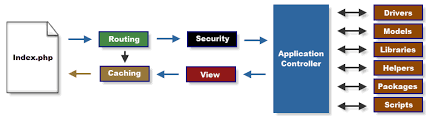
\includegraphics[scale=1.0]{appflowchart.png}  
	\caption{Flow Chart Aplikasi CodeIgniter}
	\label{fig:flowChartCodeIgniter} 
\end{figure}

\begin{enumerate}
	\item \texttt{Index.php} : bertindak sebagai \textit{front controller}, menginisiasi \textit{base resources} yang dibutuhkan untuk menjalankan CodeIgniter.
	\item \texttt{Router} : akan memeriksa permintaan HTTP untuk menetapkan hal apa yang harus dilakukan dengan permintaan tersebut.
	\item \texttt{Cache} : Apabila terdapat \textit{cache}, maka \textit{cache} tersebut akan dikirimkan langsung ke browser, dengan melewati sistem eksekusi normal.
	\item \texttt{Security} : Sebelum \textit{controller} dimuat, \textit{HTTP request} dan \textit{user} mana pun yang mengirimkan data diseleksi dahulu untuk keamanan.
	\item \texttt{Controller} : Terdiri dari \textit{model, core libraries, helpers}, dan \textit{resources} yang dibutuhkan untuk proses \textit{request} tertentu.
	\item \texttt{View} : Tampilan yang telah selesai dirubah kemudian dikirim ke \textit{web browser} untuk dilihat. Jika \textit{caching} diaktifkan, tampilan di \textit{cache} terlebih dahulu sehingga pada permintaan selanjutnya dapat dilayani.\cite{codeigniter}
\end{enumerate}

\subsection{CodeIgniter URLs}
CodeIgniter menggunakan pendekatan berbasis segmen :
\begin{lstlisting}[frame=single, language=PHP, label={lst:urlCI}, caption=Kode URLs pada CodeIgniter] 
example.com/class/function/ID
\end{lstlisting}

\begin{enumerate}
	\item Segmen pertama menyatakan kelas \textit{controller} yang harus dipanggil.
	\item Segmen kedua menyatakan fungsi kelas, atau metode, yang harus dipanggil.
	\item Segmen ketiga dan setiap segmen setelahnya menyatakan ID dan variabel apa pun yang akan diteruskan ke \textit{controller}.
\end{enumerate}

\subsection{Model}
\textit{Model} merepresentasikan struktur data. Biasanya kelas \textit {model} akan berisi fungsi yang membantu untuk \textit{retrieve, insert}, dan \textit{update} informasi di database.

\subsubsection{Anatomi Model}
Kelas model akan disimpan dalam direktori \texttt{application/models/directory}. Prototipe dasar dari sebuah model kelas :

\begin{lstlisting}[frame=single, language=PHP, label={lst:modelCI}, caption=Struktur model pada codeIgniter.]  
<?php
class Model_name extends CI_Model {

}
\end{lstlisting}

\begin{lstlisting}[frame=single, language=PHP, label={lst:userCI}, caption=Contoh model codeIgniter.]  
application/models/User_model.php
\end{lstlisting}

\subsubsection{Loading a Model}

Model akan dimuat dan dipanggil didalam metode \textit{controller}. Untuk memuat sebuah model maka dapat digunakan metode berikut:

\begin{lstlisting}[frame=single, language=PHP, label={lst:loadCI}, caption=Contoh pemanggilan model pada codeIgniter.] 
$this->load->model('model_name');
\end{lstlisting}

\subsubsection{Koneksi ke Database}
Apabila model sudah dimuat, model tersebut tidak terhubung secara langsung ke database. Dengan cara secara manual mengatur konektivitas database melalui parameter ketiga:

\begin{lstlisting}[frame=single, language=PHP, label={lst:databaseCI}, caption=Struktur database pada CodeIgniter.]
$config['hostname'] = 'localhost';
$config['username'] = 'myusername';
$config['password'] = 'mypassword';
$config['database'] = 'mydatabase';
$config['dbdriver'] = 'mysqli';
$config['dbprefix'] = '';
$config['pconnect'] = FALSE;
$config['db_debug'] = TRUE;

$this->load->model('model_name', '', $config);
\end{lstlisting}

\subsection{View}
\textit{View } adalah informasi yang disajikan kepada pengguna. Tampilan atau \textit{View} biasanya akan menjadi halaman web, tetapi dalam CodeIgniter, tampilan juga bisa berupa fragmen halaman seperti header atau footer. 

\textit{Views} tidak pernah dipanggil secara langsung, harus dimuat dalam sebuah \textit{controller}. Dalam \textit{MVC framework}, \textit{controller} bertanggung jawab untuk mengambil \textit{view} tertentu. 

\subsubsection{Membuat sebuah View}
CodeIgniter memuat view dengan memanggil sebuah file php, misalkan \verb|blogview.php|, dan \textit{developer} dapat mengisinya dengan kode HTML sebgaai berikut:
\begin{lstlisting}[frame=single, language=HTML, label={lst:viewCI}, caption=Contoh view pada CodeIgniter.] 
<html>
<head>
<title>My Blog</title>
</head>
<body>
<h1>Welcome to my Blog!</h1>
</body>
</html>
\end{lstlisting}

File tersebut akan disimpan di direktori \texttt{application/views/}.

\subsubsection{Loading sebuah View}


View dapat dimuat dengan membuat file \textit{view} dengan syntax berikut:

\begin{lstlisting}[frame=single, language=PHP, label={lst:loadViewCI}, caption=Contoh load view pada CodeIgniter.] 
$this->load->view('name');
\end{lstlisting}

\noindent Dimana \texttt{name} adalah nama dari file view.

\subsubsection{Memuat Beberapa View}

CodeIgniter dapat menangani beberapa panggilan dari dalam \textit{controller}. Apabila ada lebih dari satu panggilan yang terjadi, maka \textit{views} akan dilampirkan secara bersamaan. Berikut ini kode yang digunakan jika \textit{developer} ingin mempunyai sebuah halaman yang terdiri dari \texttt{header, menu, content} dan \texttt{footer}. 


\begin{lstlisting}[frame=single, language=PHP, label={lst:loadSomeViewCI}, caption=Contoh load beberapa view pada CodeIgniter.] 
<?php

class Page extends CI_Controller {

public function index()
{
$data['page_title'] = 'Your title';
$this->load->view('header');
$this->load->view('menu');
$this->load->view('content', $data);
$this->load->view('footer');
}

}
\end{lstlisting}

\subsubsection{Menyimpan Views didalam Sub Direktori}

Untuk menyimpan didalam sub direktori maka dapat menyertakan nama direktori yang memuat \textit{view}.
\begin{lstlisting}[frame=single, language=PHP, label={lst:loadSubDirektoriCI}, caption=Struktur penyimpanan views dalam sub direktori.] 
$this->load->view('directory_name/file_name');
\end{lstlisting}

\subsubsection{Menambahkan data dinamis ke View}

Data yang dikirim dari controller menuju view berbentuk array atau objek, sehingga akan dilampirkan dalam parameter kedua dalam metode loading view.
Kode ~\ref{lst:dynamicDataCI} menjelaskan penggunaan dengan array:
\begin{lstlisting}[frame=single, language=PHP, label={lst:dynamicDataCI}, caption=Struktur data dinamis.] 
$data = array(
'title' => 'My Title',
'heading' => 'My Heading',
'message' => 'My Message'
);

$this->load->view('blogview', $data);
\end{lstlisting}

\noindent Kemudian, penggunaan dengan objek:
\begin{lstlisting}[frame=single, language=PHP, label={lst:dynamicObjectDataCI}, caption=Struktur data dinamis berbentuk objek.] 
$data = new Someclass();
$this->load->view('blogview', $data);
\end{lstlisting}

\noindent Sehingga apabila dimasukan ke controller, kode yang ditambahkan adalah:
\begin{lstlisting}[frame=single, language=PHP, label={lst:dynamicControllerDataCI}, caption=Struktur data dinamis dalam controller.] 
<?php
class Blog extends CI_Controller {

public function index()
{
$data['title'] = "My Real Title";
$data['heading'] = "My Real Heading";

$this->load->view('blogview', $data);
}
}
\end{lstlisting}

Untuk mengaksesnya dalam file HTML maka \textit{developer} dapat menggunakan syntax php :
\begin{lstlisting}[frame=single, language=PHP, label={lst:htmlaCI}, caption=Akses data dinamis dalam file HTML.] 
<html>
<head>
<title><?php echo $title;?></title>
</head>
<body>
<h1><?php echo $heading;?></h1>
</body>
</html>
\end{lstlisting}

\subsection{Controller}
\textit{Controller} bertindak sebagai penengah antara Model, View dan \textit{resources} lain yang dibutuhkan untuk proses \textit{HTTP requests} dan untuk menghasilkan sebuah halaman web. Sebuah \textit{controller} secara sederhana merupakan sebuah file yang dinamakan dengan aturan tertentu sehingga dapat dihubungkan dengan sebuah URl.
Misalnya untuk URl ini:
\begin{lstlisting}[frame=single, language=PHP, label={lst:controllerCI}, caption=Controller pada codeIgniter.] 
<?php
example.com/index.php/blog/
\end{lstlisting}

Dalam contoh diatas, \textit{CodeIgniter} berusaha menemukan \textit{controller} bernama Blog.php dan lalu memuatnya. Ketika sebuah nama \textit{controller} sesuai dengan segmen pertama dari sebuah URl, maka URl akan memuatnya. Kode berikut merupakan contoh dari \textit{controller} sederhana.
\begin{lstlisting}[frame=single, language=PHP, label={lst:contohControllerCI}, caption=Contoh controller pada codeIgniter.] 
<?php
class Blog extends CI_Controller {

public function index()
{
echo 'Hello World'
}
}
\end{lstlisting} 

\subsubsection{Method}
Dalam sebuah kelas \textit{controller} akan memiliki beberapa method, lalu untuk memanggil fungsi didalamnya maka \textit{developer} dapat mengisi segmen kedua dari sebuah url dengan sebuah method. Misalnya controller dengan dua method yaitu \texttt{index()} dan \texttt{comments()}.
\begin{lstlisting}[frame=single, language=PHP, label={lst:methodCI}, caption=Method pada codeIgniter.] 
<?php
class Blog extends CI_Controller {

public function index()
{
echo 'Hello World!';
}

public function comments()
{
echo 'Look at this!';
}
}
\end{lstlisting}

\noindent Pemanggilan method index dapat secara otomatis dilakukan apabila segmen kedua kosong. Namun ada cara lain untuk menamplikan pesan "Hello World" yang dapat dilakukan dengan:

\begin{lstlisting}[frame=single, language=PHP, label={lst:methodCI}, caption=Method pada codeIgniter.] 
example.com/index.php/blog/index/
\end{lstlisting}

\noindent Kemudian untuk memuat method \texttt{comment()} dapat dituliskan sebagai berikut:
\begin{lstlisting}[frame=single, language=PHP, label={lst:loadMethodCI}, caption=Load method pada codeIgniter.] 
example.com/index.php/blog/comments/
\end{lstlisting}

\section{jQuery}

\begin{lstlisting}[frame=single, language=PHP, label={lst:jQuery}, caption=Load method pada codeIgniter.] 

$(document).ready(function () {
var datepickeroptions = {
format: 'Y-m-d H:i'
};
function removeRow() {
$(this).closest('.row').remove();
}
jQuery('#datetimepicker').datetimepicker();
$('#fromDateTime').datetimepicker(datepickeroptions);
$('.toDateTime').datetimepicker(datepickeroptions);
$('.eraseButton').click(removeRow);
$('select[name="changeType"]').change(function () {
$('input.disableable').removeAttr('disabled');
switch ($(this).val()) {
case 'T':
$('input[name="fromDateTime"]').attr('disabled', 'disabled');
$('input[name="fromRoom"]').attr('disabled', 'disabled');
break;
case 'X':
$('input.toDateTime').attr('disabled', 'disabled');
$('input.toRoom').attr('disabled', 'disabled');
break;
}
});
$('select[name="changeType"]').change();
var toFields = $('.toFields').clone();
$('.toFields').find('.eraseButton').remove();
$('#addToButton').click(function(e) {
e.preventDefault();
var newFields = toFields.clone();
newFields.insertBefore($('#sendDiv'));
newFields.find('.toDateTime').datetimepicker(datepickeroptions);
newFields.find('.eraseButton').click(removeRow);
});

});
\end{lstlisting}


jQuery merupakan \textit{library} Javascript dimana setiap kode yang dibuat akan disimpan ke dalam \textit{methods} yang dapat \textit{user} panggil hanya dengan satu baris kode.

\subsection{Penggunaan Dasar jQuery}
Syntax dalam jQuery dibuat untuk memilih elemen dalam HTML dan melakukan beberapa aksi dalam elemen.

Syntax dasar dalam jQuery sebagai berikut :
\begin{lstlisting}[frame=single, language=PHP, label={lst:dasarjQuery}, caption=Pemanggilan jQuery.]
$(selector).action()
\end{lstlisting}
\begin{itemize}
	\item \texttt{\$}: berfungsi untuk mendefinisikan library jQuery.
	\item \texttt{selector}: berfungsi untuk menjalankan \textit{query} atau menemukan elemen HTML.
	\item \texttt{action()}: berfungsi untuk menjalankan elemen.
\end{itemize}

Contoh penggunaan syntax dalam jQuery sebagai berikut:
\begin{itemize}
	\item \texttt{\$(this).hide()}: menyembunyikan elemen saat ini.
	\item \texttt{\$("p").hide()}: menyembunyikan elemen \texttt{<p>}.
	\item \texttt{\$(".test").hide()}: menyembunyikan elemen \texttt{class="test"}.
	\item \texttt{\$("\#test").hide()}: menyembunyikan elemen \texttt{id="test"}.
\end{itemize}
\subsection{jQuery Selectors}
\texttt{jQuery selector} memungkinkan \textit{user} untuk memilih dan memanipulasi elemen dalam HTML berdasarkan nama, id, kelas, tipe, atribut dan \textit{value} dari atribut. Semua \textit{selectors} dalam jQuery dimulai dengan simbol dollar dan tanda kurung: \texttt{\$()}.
Contoh :
Perintah user untuk memilih sebuah tombol sehingga semua elemen \texttt{<p>} akan tersembunyi.
\begin{lstlisting}[frame=single, language=PHP, label={lst:jQuerySelector}, caption=jQuery Selector pada elemen <p>.]	
$(document).ready(function(){
$("button").click(function(){
$("p").hide();
});
});

\end{lstlisting}

\subsection{jQuery Event}
Semua aksi yang dilakukan \textit{user} dalam web dapat direspon oleh sistem yang dinamakan \textit{events}. Events menunjukkan momen apabila suatu kegiatan terjadi seperti: memindahkan mouse ke sebuah elemen, memilih sebuah radio button dan menekan sebuah elemen.

\subsubsection{\texttt{\$(document).ready}}
Seluruh metode jQuery akan berada didalam sebuah \texttt{document ready event} :
%.ready()
\begin{lstlisting}[frame=single, language=PHP, label={lst:jQueryReady}, caption=jQuery document ready event.]
$(document).ready(function(){
// jQuery methods go here...
});
\end{lstlisting}

Syntax ~\ref{lst:jQueryReady} untuk menghindari kode jQuery berjalan sebelum dokumen siap untuk di-\textit{load}. Contoh aksi yang akan gagal apabila kode berjalan sebelum dokumen siap seperti:
\begin{itemize}
	\item Mencoba untuk menghilangkan elemen yang belum selesai dibuat.
	\item Mencoba untuk mendapatkan ukuran gambar yang belum di-\textit{load} seluruhnya.
\end{itemize}


%.click
\subsubsection{\texttt{click()}}
Metode \texttt{click()} melampirkan fungsi event handler ke elemen HTML, sehingga fungsi akan dieksekusi ketika \textit{user} mengklik elemen HTML.
Contoh : Memilih elemen \texttt{<p>} untuk memberikan teks berupa alert
\begin{lstlisting}[frame=single, language=PHP, label={lst:jQueryClick}, caption=jQuery click().]
$("p").click(function(){
alert("The paragraph was clicked.");
});

\end{lstlisting}

%.change()
\subsubsection{\texttt{change()}}
Metode \texttt{change()} akan memicu perubahan ketika kode dijalankan. Change event hanya bisa merubah elemen \texttt{<input>,<textarea>} dan \texttt{<select>}.
Ada dua syntax yang dipakai :
\begin{itemize}
	\item \texttt{\$(selector).change()}: memicu perubahan event untuk elemen terpilih.
	\item \texttt{\$(selector).change(function)}: memicu perubahan event dengan menerapkan fungsi tertentu.
\end{itemize}
Contoh penggunaan metode ini: Memberikan teks peringatan ketika sebuah field \texttt{<input>} berubah.
\begin{lstlisting}[frame=single, language=PHP, label={lst:jQueryChange}, caption=jQuery change().]
$("input").change(function(){
alert("The text has been changed.");
});
\end{lstlisting}

%.select()
\subsubsection{\texttt{select()}}
Event select akan memilih teks terpilih di dalam text area atau text field.
Metode \texttt{select()} memicu event atau fungsi untuk berjalan ketika sebuah event terpilih dijalankan.
Ada dua syntax yang dipakai :
\begin{itemize}
	\item \texttt{\$(selector).select()}: memicu perubahan event untuk elemen terpilih.
	\item \texttt{\$(selector).select(function)}: memicu perubahan event dengan menerapkan fungsi tertentu.
\end{itemize}
Contoh penggunaan metode : Memberikan sebuah peringatan ketika sebuah teks dipilih didalam sebuah \textit{text field}.
\begin{lstlisting}[frame=single, language=PHP, label={lst:jQuerySelect}, caption=jQuery Selector.]
$("input").select(function(){
alert("Text marked!");
});
\end{lstlisting}

\subsubsection{\texttt{preventDefault()}}
Metode preventDefault() membatalkan event yang \textit{user} kehendaki. Apabila terdapat sebuah link, maka user tidak bisa menuju link tersebut. Atau apabila ada button "Submit" dalam sebuah form, maka user tidak bisa mengumpulkan form tersebut.
\begin{lstlisting}[frame=single, language=javascript, label={lst:jQuerypreventDefault}, caption=jQuery preventDefault().]
document.getElementById("myAnchor").addEventListener("click", 
function(event){
event.preventDefault()
});
\end{lstlisting}


\subsection{jQuery Traversing}
Berfungsi untuk menemukan elemen HTML berdasarkan relasinya dengan elemen lain. Metode yang dipakai untuk fungsi ~\ref{fig:jQueryClosest} adalah:
\subsubsection{\texttt{closest()}}
Fungsi \texttt{closest()} akan mengembalikan \textit{ancestor} pertama dari elemen terpilih.
%.closest()
\begin{figure} [H]
	\centering  
	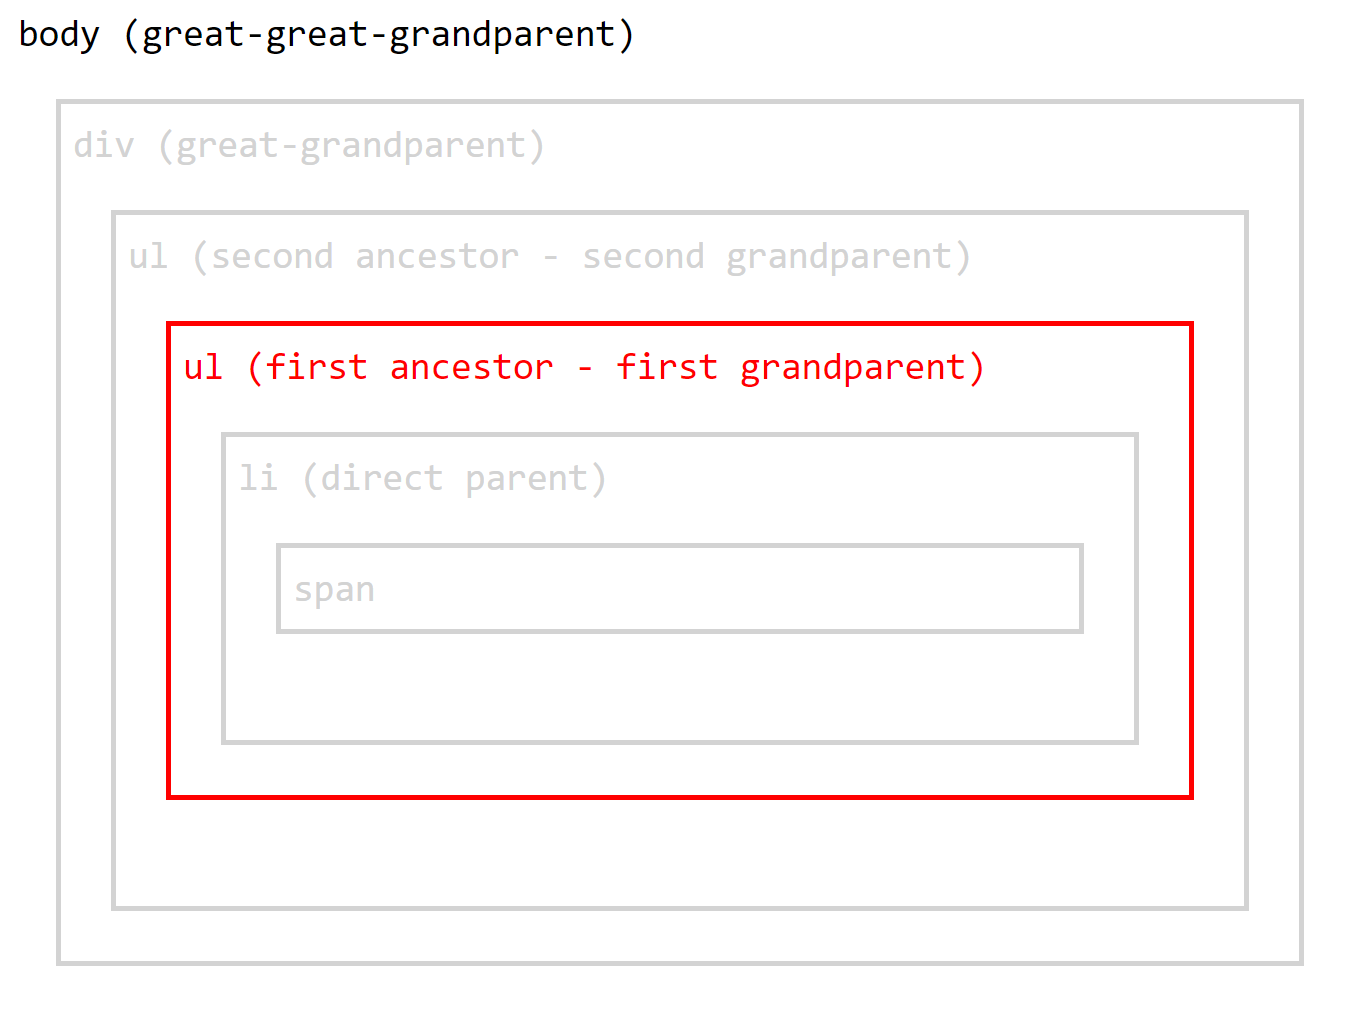
\includegraphics[scale=1.0]{jQuery_closest.png}  
	\caption{jQuery Closest} 
	\label{fig:jQueryClosest}
\end{figure}

\begin{lstlisting}[frame=single, language=jquery, breaklines=true, label={lst:jQueryClosest}, caption=jQuery Closest.]
$(document).ready(function(){
$("span").closest("ul").css({"color": "red", "border": "2px solid red"});
});
\end{lstlisting}

Kode ~\ref{lst:jQueryClosest} akan mengembalikan \textit{ancestor} dari \texttt{<span>}, yaitu sebuah elemen \texttt{<ul>}.
Hasil :
%Gambar jQuery_closest

%.find()
\subsubsection{\texttt{find()}}
Metode \texttt{find()} mengembalikan elemen turunan/descendant dari elemen yang dipilih oleh \textit{user}.
Contoh: Mengembalikan semua elemen \texttt{<span>} yang merupakan turunan dari elemen \texttt{<ul>}.
%.closest()


\begin{lstlisting}[frame=single,language=PHP, breaklines=true, label={lst:jQueryFind}, caption=jQuery find().]
$(document).ready(function(){
$("ul").find("span").css({"color": "red", "border": "2px solid red"});
});
\end{lstlisting}

Hasil dari kode  ~\ref{lst:jQueryfind} terlihat pada gambar ~\ref{fig:jQueryfind}: 
\begin{figure} [H]
	\centering  
	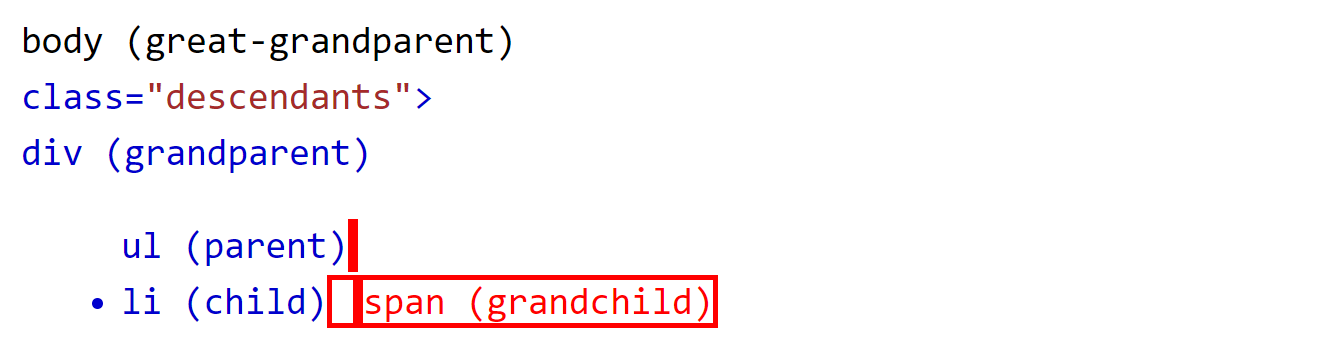
\includegraphics[scale=1.0]{jQuery_find.png}  
	\caption{jQuery Find} 
	\label{fig:jQueryfind}
\end{figure}


\subsection{jQuery HTML}
%.remove()
\subsubsection{\texttt{remove()}}
\texttt{remove()} - berfungsi untuk menghapus elemen HTML yang ada. Contoh penggunaan nya seperti:
Menghapus elemen dengan \texttt{id="div1"}.
\begin{lstlisting} [frame=single, language=PHP, label={lst:jQueryRemove}, caption=jQuery remove().]
$("#div1").remove();
\end{lstlisting}

%.removeAttr()
\subsubsection{\texttt{\$removeAttr()}}
Metode \texttt{removeAttr()} menghapus satu atau banyak atribut dari elemen terpilih.
Syntax dari metode ini :
\begin{lstlisting}[frame=single, language=jQuery, , label={lst:jQueryRemoveAttr}, caption=jQuery removeAttr().]
$(selector).removeAttr(attribute)
\end{lstlisting}

Contoh pemakaian metode ini: Menghapus atribut style dari semua elemen <p>:
\begin{lstlisting}[frame=single, language=jquery, label={lst:contohjQueryRemoveAttr}, caption=contoh jQuery removeAttr().]
$("button").click(function(){
$("p").removeAttr("style");
});
\end{lstlisting}

%.clone()
\subsubsection{\texttt{\$clone()}}
Metode \texttt{clone()} membuat salinan dari elemen terpilih, termasuk child nodes, teks atau atribut.
Syntax dari metode ini :
\begin{lstlisting} [frame=single, language=PHP, label={lst:jQueryClone}, caption=jQuery clone().]
$(selector).clone(true|false))
\end{lstlisting}

Contoh pemakaian metode ini: Clone semua elemen \texttt{<p>} dan masukan semua elemen pada akhir elemen \texttt{<body>}.
\begin{lstlisting}[frame=single, language=PHP, label={lst:contohjQueryClone}, caption=contoh jQuery clone().]
$("button").click(function(){
$("p").clone().appendTo("body");
});
\end{lstlisting}


%.insertBefore
\subsubsection{\texttt{insertBefore()}}
Metode \texttt{insertBefore()} akan memasukan elemen HTML sebelum elemen terpilih.
Syntax dari metode ini :
\begin{lstlisting} [frame=single, language=PHP, label={lst:jQueryInsertBefore}, caption=insertBefore().]
$(content).insertBefore(selector)
\end{lstlisting}
Dimana :
\begin{itemize}
	\item \texttt{content} : \texttt{Required}. Detail konten yang harus dimasukan (harus berisi tags HTML).
	\item \texttt{selector} : \texttt{Required}. Menjelaskan dimana konten akan dimasukan. 
\end{itemize}

Contoh pemakaian metode ini: Memasukkan sebuah elemen \texttt{<span>} sebelum \texttt{<p>}.
\begin{lstlisting}[frame=single, language=PHP, label={lst:jQueryinsertBefore}, caption=jQuery insertBefore().]
$("button").click(function(){
$("<span>Hello world!</span>").insertBefore("p");
});
\end{lstlisting}

\section{Foundation 6}
\subsection{Struktur File}
\begin{lstlisting}[basicstyle=\ttfamily, frame=single,
columns=fullflexible, keepspaces=true, breaklines=true, label={lst:fileFoundation}, caption=Struktur File Foundation.]
.
|-- css
|   |-- css 
|   |-- foundatcss 
|   |-- foundation-datetimepicker.css 
|   |-- foundation-fcss 
|   |-- foundation-icss 
|   |-- foundation-ieot 
|   |-- foundation-isvg 
|   |-- foundation-ittf 
|   |-- foundation-icoff 
|-- js
|   |-- vendor 
|   |-- app.js 
|   |-- foundation.js 
|-- img
.
\end{lstlisting}

Framework Foundation terdiri dari 3 folder utama:
\begin{itemize}
	\item Folder \texttt{css} terdiri dari semua \textit{CSS Style} yang digunakan dalam Foundation 6. Didalam folder terdapat versi yag diperkecil yaitu \verb|foundation.min.css| atau versi yang tidak dikompresi \verb|foundation.css|. Lalu seluruh modifikasi \textit{stylesheets} ditempatkan didalam folder ini agar lebih terstruktur.
	\item Folder \texttt{img} tempat meletakkan semua gambar untuk projek web.
	\item Folder \texttt{js} terdiri dari semua file Javascript.
\end{itemize} 
\cite{zurbfoundation:17}

\subsection{Sistem Grid}
Penggunaan grid pada Foundation dapat dilakukan dengan menambahkan sebuah elemen dengan sebuah kelas \texttt{.row} sehingga akan membuat blok horizontal yang berisi kolom vertikal. Kemudian kelas \texttt{.column} akan ditambahkan pada baris tersebut, lalu masing-masing kolom ditentunkan kelasnya dengan tiga pilihan yaitu 
\texttt{.small-\#}, \texttt{.medium-\#} dan \texttt{.large-\#}.

\begin{lstlisting}[language=HTML,  basicstyle=\ttfamily, frame=single, columns=fullflexible, keepspaces=true, breaklines=true, showstringspaces=false, label={lst:gridFoundation}, caption=Struktur Grid Foundation 6.] 
<div class="row">
<div class="columns small-2 large-4"><!-- ... --></div>
<div class="columns small-4 large-4"><!-- ... --></div>
<div class="columns small-6 large-4"><!-- ... --></div>
</div>
<div class="row">
<div class="columns large-3"><!-- ... --></div>
<div class="columns large-6"><!-- ... --></div>
<div class="columns large-3"><!-- ... --></div>
</div>
<div class="row">
<div class="columns small-6 large-2"><!-- ... --></div>
<div class="columns small-6 large-8"><!-- ... --></div>
<div class="columns small-12 large-2"><!-- ... --></div>
</div>
<div class="row">
<div class="columns small-3"><!-- ... --></div>
<div class="columns small-9"><!-- ... --></div>
</div>
<div class="row">
<div class="columns large-4"><!-- ... --></div>
<div class="columns large-8"><!-- ... --></div>
</div>
<div class="row">
<div class="columns small-6 large-5"><!-- ... --></div>
<div class="columns small-6 large-7"><!-- ... --></div>
</div>
<div class="row">
<div class="columns large-6"><!-- ... --></div>
<div class="columns large-6"><!-- ... --></div>
</div>
\end{lstlisting}

\begin{figure} [H]
	\centering  
	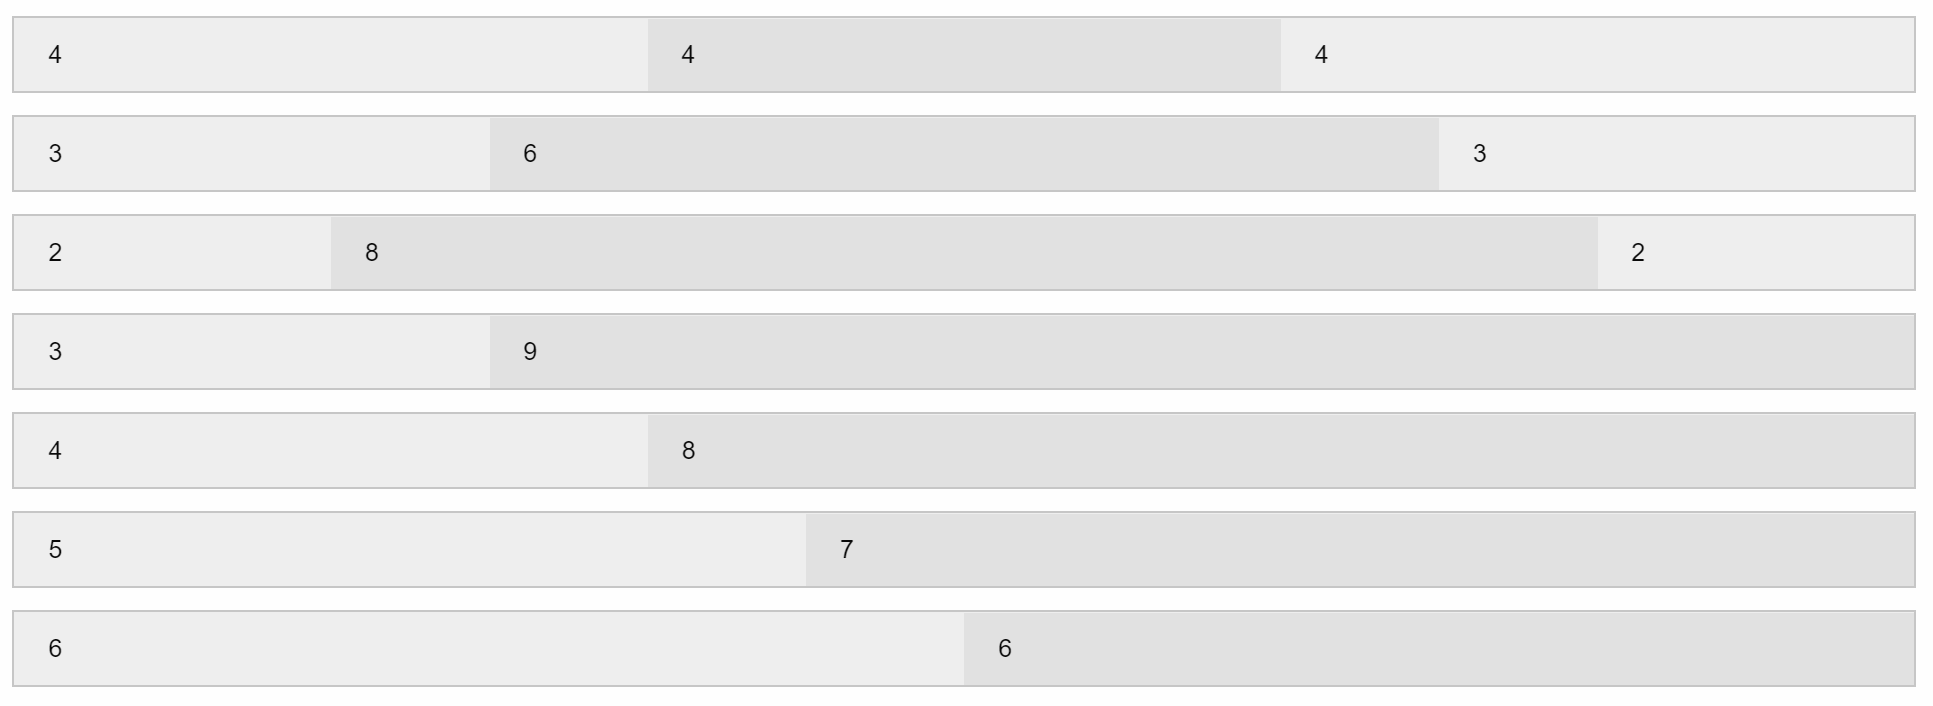
\includegraphics[scale=0.7]{gridbasic_zurb.png}  
	\caption{Grid pada Zurb Foundation}
	\label{fig:gridFoundation}	 
\end{figure}

\subsection{Navigation dan Media Attributes}
Komponen menu yang fleksibel pada Foundation membuat pembangunan navigasi secara umum lebih mudah karena semua pola memiliki markup yang sama.

\subsubsection{Basic Menu}

Menu terdiri dari sebuah \texttt{<ul>} yang diisi oleh beberapa tag \texttt{<li>}. Secara default, menu akan berorientasi horizontal.

Berikut ini contoh penggunaan kode navigasi pada menu:

\begin{lstlisting}[language=HTML,  basicstyle=\ttfamily, frame=single, columns=fullflexible, keepspaces=true, breaklines=true, showstringspaces=false, label={lst:basicFoundation}, caption=Basic Menu Foundation 6.] 
<ul class="menu">
<li><a href="#">One</a></li>
<li><a href="#">Two</a></li>
<li><a href="#">Three</a></li>
<li><a href="#">Four</a></li>
</ul>
\end{lstlisting}

\begin{figure} [H]  
	\centering  
	
\includegraphics[scale=0.7]{basicmenu_zurb.png}  
	\caption{\textit{Basic Navigation Menu} pada Foundation}
	\label{fig:navFoundation}
\end{figure}

\subsubsection{Item Alignment}
Secara default, setiap item dalam menu akan berlajur ke arah kiri. Menu dapat diubah lajurnya ke arah kanan dengan menggunakan kelas \texttt{.align-right} atau kearah tengah dengan menambahkan kelas \texttt{.align-center} didalam kelas \texttt{.menu}.
\begin{lstlisting}[language=HTML,  basicstyle=\ttfamily, frame=single, columns=fullflexible, keepspaces=true, breaklines=true, showstringspaces=false, label={lst:itemAlignmentFoundation}, caption=Item Alignment Foundation 6.] 
<ul class="menu align-right">
<li><a href="#">One</a></li>
<li><a href="#">Two</a></li>
<li><a href="#">Three</a></li>
<li><a href="#">Four</a></li>
</ul>
\end{lstlisting}

\begin{figure}[H]
	\centering  
	
\includegraphics[scale=0.7]{basicmenu_right_zurb.png}  
	\caption{Menu \textit{align to right} dalam Foundation}
	\label{fig:alignRightFoundation}
\end{figure}

\begin{lstlisting}[language=HTML,  basicstyle=\ttfamily, frame=single, columns=fullflexible, keepspaces=true, breaklines=true, showstringspaces=false, label={lst:aligntorightFoundation}, caption=Align to right Foundation 6.] 
<ul class="menu align-center">
<li><a href="#">One</a></li>
<li><a href="#">Two</a></li>
<li><a href="#">Three</a></li>
<li><a href="#">Four</a></li>
</ul>
\end{lstlisting}

\begin{figure} [H]
	\centering  
	
\includegraphics[scale=0.7]{basicmenuCenter_zurb.png}  
	\caption{Menu \textit{align to center} dalam Foundation}
	\label{fig:alignCenterFoundation}
\end{figure}

\subsubsection{Active State}
Kelas \texttt{.is-active} dapat ditambahkan ke dalam tag \texttt{<li>} untuk membuat menu terpilih yang aktif terlihat saat di klik. 

\begin{lstlisting}[language=HTML,  basicstyle=\ttfamily, frame=single, columns=fullflexible, keepspaces=true, breaklines=true, showstringspaces=false, label={lst:activeStateFoundation}, caption=Active State Foundation 6.] 
<ul class="menu">
<li class="is-active"><a>Home</a></li>
<li><a>About</a></li>
<li><a>Nachos</a></li>
</ul>
\end{lstlisting}

\begin{figure} [H]
	\centering  
	
\includegraphics[scale=0.7]{activestatemenu_zurb.png}  
	\caption{Menu \textit{active state} dalam Foundation}
	\label{fig:activeStateFoundation}
\end{figure}


\subsubsection{Text}
Karena \textit{padding} untuk setiap item menu menggunakan tag \texttt{<a>}, maka apabila sebuah item yang hanya berisi teks, maka teks tersebut tidak selaras dengan item menu lainnya. Sehingga untuk menyiasatinya, dapat menggunakan kelas \texttt{.menu-text} yang dituliskan dalam tag \textit{<li>} dengan menyertakan sebuah teks tanpa link.

\begin{lstlisting}[language=HTML,  basicstyle=\ttfamily, frame=single, columns=fullflexible, keepspaces=true, breaklines=true, showstringspaces=false, label={lst:textFoundation}, caption=Text Foundation 6.]
<ul class="menu">
<li class="menu-text">Site Title</li>
<li><a href="#">One</a></li>
<li><a href="#">Two</a></li>
<li><a href="#">Three</a></li>
</ul>
\end{lstlisting}

\begin{figure} [H]
	\centering  
	
\includegraphics[scale=0.7]{menutext_zurb.png}  
	\caption{\textit{Menu text} dalam Foundation}
	\label{fig:menuTextFoundation}
\end{figure}

\subsection{Komponen}

\subsubsection{Button}
\textit{Basic button} dapat digunakan untuk banyak tujuan, sehingga penting untuk \textit{developer} menggunakan tag yang tepat. Berikut ini penjelasan penggunaan \textit{Basic button} dalam Foundation
\begin{itemize}
	\item Penggunaan tag \texttt{<a>} digunakan apabila tombol memiliki \textit{link} ke halaman lain, atau \textit{link} menuju ke halaman itu sendiri. Penggunaan links tidak membutuhkan JavaScript.
	\item Penggunaan tag \texttt{<button>} jika tombol melakukan tindakan yang mengubah sesuatu pada halaman seperti proses \textit{delete} atau \textit{save}. Elemen \texttt{<button>} akan membutuhkan JavaScript agar proses tersebut berfungsi. 
\end{itemize}

\begin{lstlisting}[language=HTML,  basicstyle=\ttfamily, frame=single, columns=fullflexible, keepspaces=true, breaklines=true, showstringspaces=false, label={lst:buttonFoundation}, caption=Button pada foundation 6.] 
<!-- Anchors (links) -->
<a href="about.html" class="button">Learn More</a>
<a href="#features" class="button">View All Features</a>

<!-- Buttons (actions) -->
<button type="button" class="success button">Save</button>
<button type="button" class="alert button">Delete</button>
\end{lstlisting}

\begin{figure} [H]
	\centering  
	
\includegraphics[scale=0.7]{basicbutton_zurb.png}  
	\caption{Basic Button pada Foundation}
	\label{fig:buttonFoundation}
\end{figure}

\noindent Warna pada button dapat diterapkan untuk memperlihatkan fungsi yang sesuai dengan aksi yang digunakan.
\begin{lstlisting}[language=HTML,  basicstyle=\ttfamily, frame=single, columns=fullflexible, keepspaces=true, breaklines=true, showstringspaces=false, label={lst:basicButtonFoundation}, caption=Basic Button pada foundation 6.] 
<a class="button primary" href="#">Primary</a>
<a class="button secondary" href="#">Secondary</a>
<a class="button success" href="#">Success</a>
<a class="button alert" href="#">Alert</a>
<a class="button warning" href="#">Warning</a>
\end{lstlisting}

\begin{figure} [H]
	\centering  
	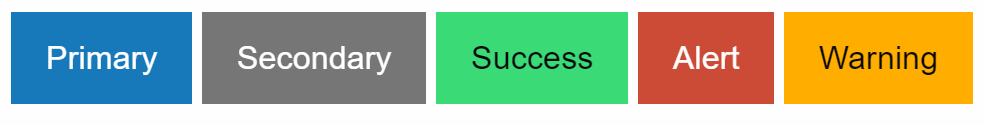
\includegraphics[scale=0.7]{coloringbutton_zurb.png}  
	\caption{Coloring Button pada Foundation}
	\label{fig:colorButtonFoundation}
\end{figure}

\subsubsection{Tabel}

Tabel dalam foundation akan menjadikan proses penampilan data bersifat responsif dan memiliki tata letak yang bisa disesuaikan oleh kebutuhan \textit{developer}.


\begin{lstlisting}[language=HTML,  basicstyle=\ttfamily, frame=single, columns=fullflexible, keepspaces=true, breaklines=true, showstringspaces=false, label={lst:tabelFoundation}, caption=Tabel pada foundation 6.]  
<table>
<thead>
<tr>
<th width="200">Table Header</th>
<th>Table Header</th>
<th width="150">Table Header</th>
<th width="150">Table Header</th>
</tr>
</thead>
<tbody>
<tr>
<td>Content Goes Here</td>
<td>This is longer content Donec id elit non mi porta gravida at eget metus.</td>
<td>Content Goes Here</td>
<td>Content Goes Here</td>
</tr>
<tr>
<td>Content Goes Here</td>
<td>This is longer Content Goes Here Donec id elit non mi porta gravida at eget metus.</td>
<td>Content Goes Here</td>
<td>Content Goes Here</td>
</tr>
<tr>
<td>Content Goes Here</td>
<td>This is longer Content Goes Here Donec id elit non mi porta gravida at eget metus.</td>
<td>Content Goes Here</td>
<td>Content Goes Here</td>
</tr>
</tbody>
</table>
\end{lstlisting}

\begin{figure} [H]
	\centering  
	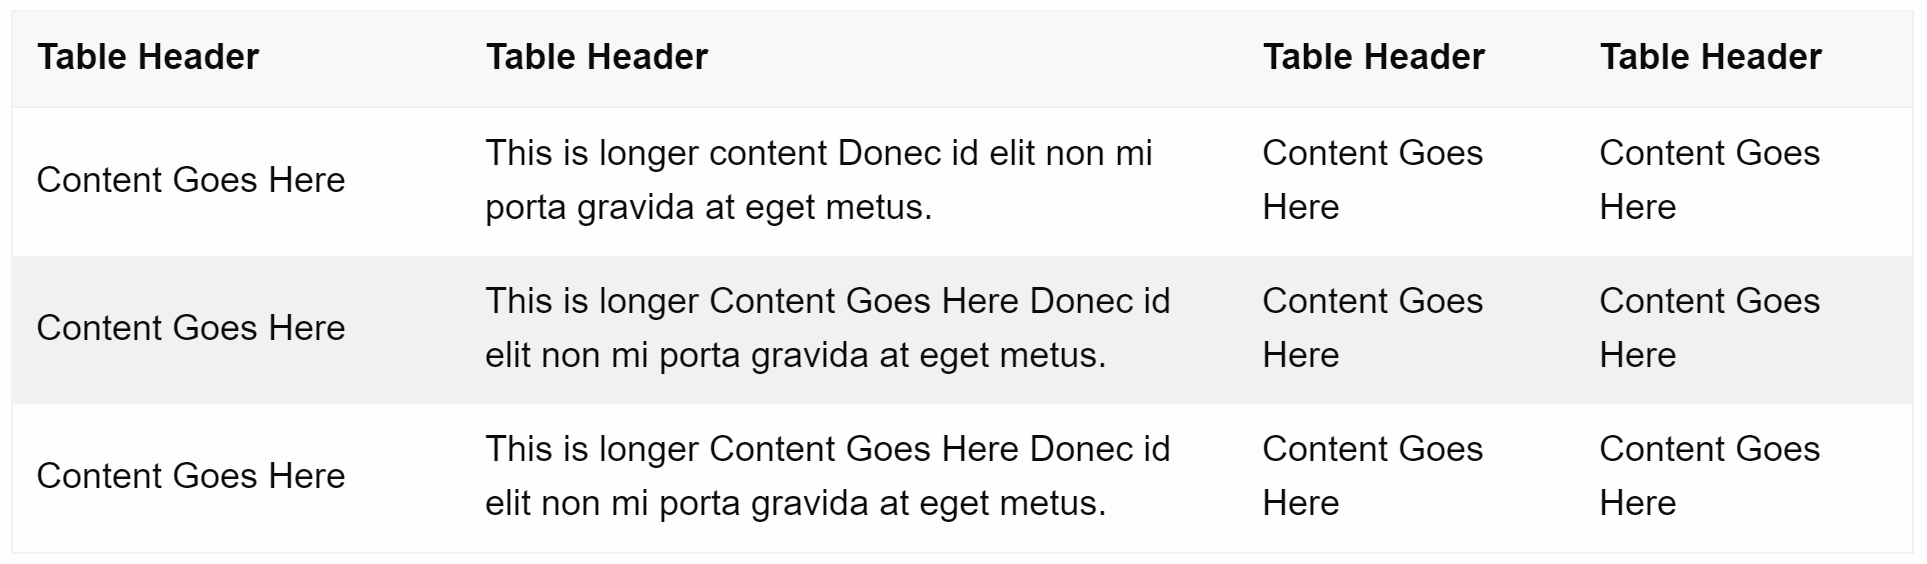
\includegraphics[scale=0.7]{basictable_zurb.png}  
	\caption{Basic Table pada Foundation}
	\label{fig:tableFoundation}
\end{figure}

\subsubsection{Hover State}
Hover State diaplikasikan menggunakan kelas \texttt{.hover} untuk sedikit membedakan baris terpilih dalam tabel dengan baris-baris lainnya dengan cara menggelapkan baris terpilih.
\begin{lstlisting}[language=HTML,  basicstyle=\ttfamily, frame=single, columns=fullflexible, keepspaces=true, breaklines=true, showstringspaces=false, label={lst:hoverstateFoundation}, caption=Hover State pada foundation 6.] 
<table class="hover">
</table>
\end{lstlisting}

\subsubsection{Striped}
Secara default, tabel akan memiliki baris yang bergaris. 
Ada beberapa pilihan kelas untuk mengubah desain tabelnya.
\begin{itemize}
	\item Kelas \texttt{.unstriped} dapat digunakan untuk menghapus garis-garis atau dengan mengubah \verb|$table-is-striped| ke \textit{false} untuk menghapus semua strip pada seluruh tabel.
	\item Kelas \texttt{.striped} untuk menambahkan strip pada tabel.	
\end{itemize}

\subsubsection{Forms}
\texttt{Forms} pada Foundation dibuat dengan kombinasi standar dari elemen \texttt{form}, serta \textit{grid rows} dan \textit{columns} atau \textit{cells}. 

\paragraph{Text Inputs}
Kode berikut ini akan membuat sebuah \textit{text field} yang bisa diterapkan untuk \textit{field} : \texttt{text, date, datetime, datetime-local, email, month, number, password, search, tel, time, url,} dan \texttt{week}.

\begin{lstlisting}[language=HTML,  basicstyle=\ttfamily, frame=single, columns=fullflexible, keepspaces=true, breaklines=true, showstringspaces=false, label={lst:textinputsFoundation}, caption=Text inputs pada foundation 6.] 
<form>
<div class="grid-container">
<div class="grid-x grid-padding-x">
<div class="medium-6 cell">
<label>Input Label
<input type="text" placeholder=".medium-6.cell">
</label>
</div>
<div class="medium-6 cell">
<label>Input Label
<input type="text" placeholder=".medium-6.cell">
</label>
</div>
</div>
</div>
</form>
\end{lstlisting}

\begin{figure} [H]
	\centering  
	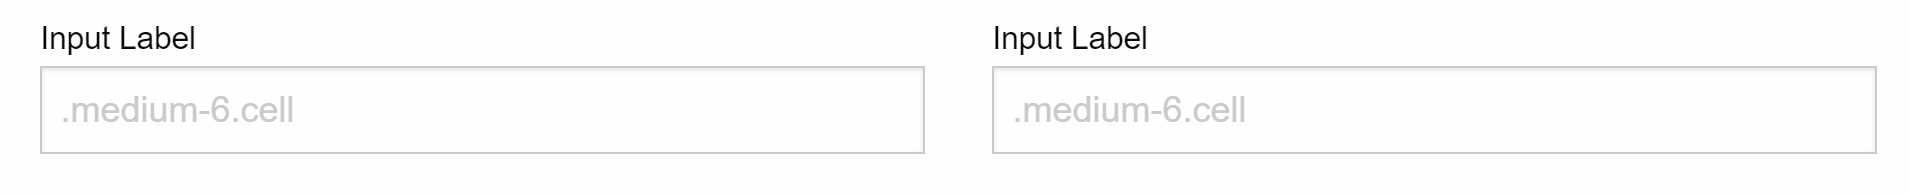
\includegraphics[scale=0.7]{input_zurb.png}  
	\caption{Text Input pada Foundation}
	\label{fig:gridbasicZurb} 
\end{figure}

\paragraph{Select Menus}
Penggunaan \texttt{select menus} digunakan apabila \textit{developer} menginginkan banyak pilihan data dalam satu menu.
\begin{lstlisting}[language=HTML,  basicstyle=\ttfamily, frame=single, columns=fullflexible, keepspaces=true, breaklines=true, showstringspaces=false, label={lst:selectMenusFoundation}, caption=Select menus pada foundation 6.] 
<label>Select Menu
<select>
<option value="husker">Husker</option>
<option value="starbuck">Starbuck</option>
<option value="hotdog">Hot Dog</option>
<option value="apollo">Apollo</option>
</select>
</label>
\end{lstlisting}


\subsubsection{Tabs}
Tab semakin banyak digunakan dalam desain web karena \textit{developer} dapat menyajikan konten secara seragam. Ini memungkinkan \textit{developer} untuk menyimpan banyak dokumen dalam satu \textit{window}. \textit{developer} dapat menggunakan tab sebagai widget navigasi untuk beralih antar konten sehingga menghasilkan tata letak yang sistematis dan bersih. Komponen Tab dari Foundation membantu \textit{developer} melakukan hal itu hanya dengan menambahkan beberapa baris kode. 

\begin{lstlisting}[language=HTML,  basicstyle=\ttfamily, frame=single, columns=fullflexible, keepspaces=true, breaklines=true, showstringspaces=false, label={lst:tabsFoundation}, caption=Tabs pada foundation 6.] 
<ul class="tabs" data-tabs id="tab_component">
<li class="tabs-title"><a href="#pub1">Section 1</a></li>
<li class="tabs-title is-active"><a href="#pub2">Section 2</a></li>
<li class="tabs-title"><a href="#pub3">Section 3</a></li>
<li class="tabs-title"><a href="#pub4">Section 4</a></li>
</ul>
<div class="tabs-content" data-tabs-content="tab_component">
<div class="tabs-panel" id="pub1">
<p>Far far away, behind the word mountains, far from the countries
Vokalia and Consonantia, there live the blind texts.</p>
</div>
<div class="tabs-panel is-active" id="pub2">
<p> Separated they live in Bookmarksgrove right at the coast of the
Semantics, a large language ocean. </p>
</div>
<div class="tabs-panel" id="pub3">
<p>A small river named Duden flows by their place and supplies it with
the necessary regelialia.</p>
</div>
<div class="tabs-panel" id="pub4">
<p>It is a paradisematic country, in which roasted parts of sentences
fly into your mouth. </p>
</div>
</div>
\end{lstlisting}

\begin{figure} [H]
	\centering  
	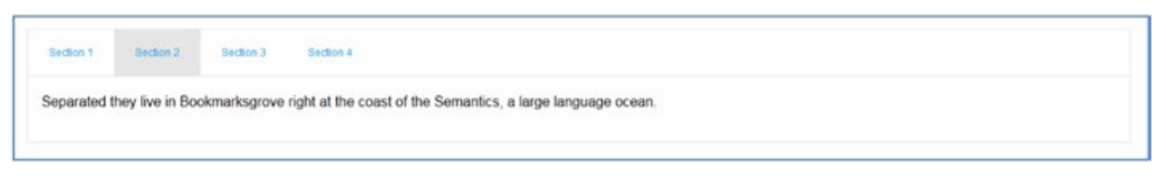
\includegraphics[scale=0.7]{tabs_component_zurb.png}  
	\caption{Tabs pada Foundation 6}
	\label{fig:tabsFoundation}
\end{figure}

\subsubsection{Dropdown Menu}
Berfungsi untuk mengubah menu dasar menjadi menu dropdown yang dapat di-expand dengan plugin Menu Dropdown.
Menu dropdown dibangun berdasarkan sintaks komponen \texttt{Menu}. Tambahkan kelas \texttt{.dropdown} dan atribut \texttt{data-dropdown-menu} ke wadah menu untuk mengatur dropdown. 
\begin{lstlisting}[language=HTML,  basicstyle=\ttfamily, frame=single, columns=fullflexible, keepspaces=true, breaklines=true, showstringspaces=false, label={lst:dropdownMenuFoundation}, caption=Dropdown menu pada foundation 6.] 
<ul class="dropdown menu" data-dropdown-menu>
<li><a href="#">Item 1</a></li>
<li><a href="#">Item 2</a></li>
<li><a href="#">Item 3</a></li>
<li><a href="#">Item 4</a></li>
</ul>
\end{lstlisting}

\subsubsection{Reveal}
Modal hanyalah wadah kosong, sehingga \textit{developer} dapat menaruh segala jenis konten di dalamnya, seperti teks ke formulir hingga video ke seluruh \textit{grid}.
Untuk membuat modal, tambahkan kelas \texttt{.reveal}, atribut \texttt{data-reveal}, dan ID yang unik ke dalam \textit{container}.

\begin{lstlisting}[language=HTML,  basicstyle=\ttfamily, frame=single, columns=fullflexible, keepspaces=true, breaklines=true, showstringspaces=false, label={lst:revealFoundation}, caption=Reveal pada foundation 6.]  
<div class="reveal" id="exampleModal1" data-reveal>
<h1>Awesome. I Have It.</h1>
<p class="lead">Your couch. It is mine.</p>
<p>I'm a cool paragraph that lives inside of an even cooler modal. Wins!</p>
<button class="close-button" data-close aria-label="Close modal" type="button">
<span aria-hidden="true">&times;</span>
</button>
</div>
\end{lstlisting} 

\section{Bootstrap 4}
\subsection{Struktur File}
\begin{lstlisting}[basicstyle=\ttfamily, frame=single,
columns=fullflexible, keepspaces=true, breaklines=true, label={lst:strukturBootstrap}, caption=Struktur file pada bootstrap 4]
.bootstrap/
|-- css/
|   |-- bootstrap.css 
|   |-- bootstrap.min.css 
|-- js/
|   |-- bootstrap.js
|   |-- bootstrap.min.js
|-- img/
|-- glyphicons-halflings.png
|-- glyphicons-halflings-white.png
.
\end{lstlisting}
Folder Bootstrap 4 berisi \textit{compiled file}(\texttt{bootstrap.min.*}) dan versi mini (\texttt{bootstrap.min.*}) dalam format \texttt{css} dan \texttt{js}. Kemudian ada folder \texttt{img} untuk simpan gambar.

\subsection{Sistem Grid}
Sistem grid Bootstrap menggunakan \textit{container}, \textit{rows}, dan \textit{columns} untuk tata letak dan penyelarasan konten. Selain itu sistem ini dibangun dengan \textit{flexbox} dan seluruhnya \textit{responsive}. \cite{bootstrap:19}
\begin{figure} [H]
	\centering  
	
\includegraphics[scale=0.7]{gridbasic_bootstrap.png}  
	\caption{Grid pada Bootstrap} 
	\label{fig:gridBootstrap}
\end{figure}

\begin{lstlisting}[language=HTML,  basicstyle=\ttfamily, frame=single, columns=fullflexible, keepspaces=true, breaklines=true, showstringspaces=false, label={lst:gridBootstrap}, caption=Sistem grid pada bootstrap 4] 
<div class="container">
<div class="row">
<div class="col-sm">
One of three columns
</div>
<div class="col-sm">
One of three columns
</div>
<div class="col-sm">
One of three columns
</div>
</div>
</div>
\end{lstlisting}
Dalam contoh diatas akan dibuat tiga kolom yang memiliki lebar yang sama baik dalam \textit{device} \textit{small, medium, large} dan \textit{extra large} menggunakan kelas grid yang sudah ditentukan sebelumnya oleh Bootstrap. Penggunaan \verb|.container| akan membuat kolom berada ditengah halaman.

Secara detil, bootstrap bekerja dengan cara:
\begin{itemize}
	\item \textit{Container} disediakan agar konten berada ditengah halaman dan mengisi konten tersebut secara horizontal. Penggunaan \verb|.container| untuk menentukan lebar pixel secara responsif atau \verb|.container-fluid| untuk membuat lebar: 100\%  di semua ukuran \textit{viewport} dan perangkat.
	\item Sebuah baris akan membungkus kolom - kolom. Setiap kolom akan memiliki \textit{padding} secara horizontal yang disebut \verb|gutter| untuk mengatur jarak antar kolom.
	\item Penggunaan flexbox akan membuat lebar pada kolom tidak perlu dispesifikasikan. Misalnya empat variabel dari \verb|.com-sm| akan secara otomatis membuat lebar kolom sebesar 25\%.
	\item Kelas kolom menunjukkan jumlah kolom yang ingin digunakan, dengan maksimal 12 kolom per baris. Apabila \textit{developer} menginginkan tiga kolom yang memiliki lebar yang sama maka dapat menggunakan \texttt{.col-4}.
	\item Lebar kolom diatur dalam persentase, sehingga kolom akan memiliki lebar yang berubah-ubah dan ukuran bergantung dengan elemen \textit{parent} nya.
\end{itemize}
\subsubsection{Pilihan Grid}
Bootstrap menggunakan px untuk grid breakpoint dan lebar container. Ini dikarenakan lebar \textit{viewport} ditentukan denga satuan pixels.
Berikut ini tabel yang menjelaskan penggunaan kelas grid dalam berbagai perangkat :
\begin{figure} [H]
	\centering  
	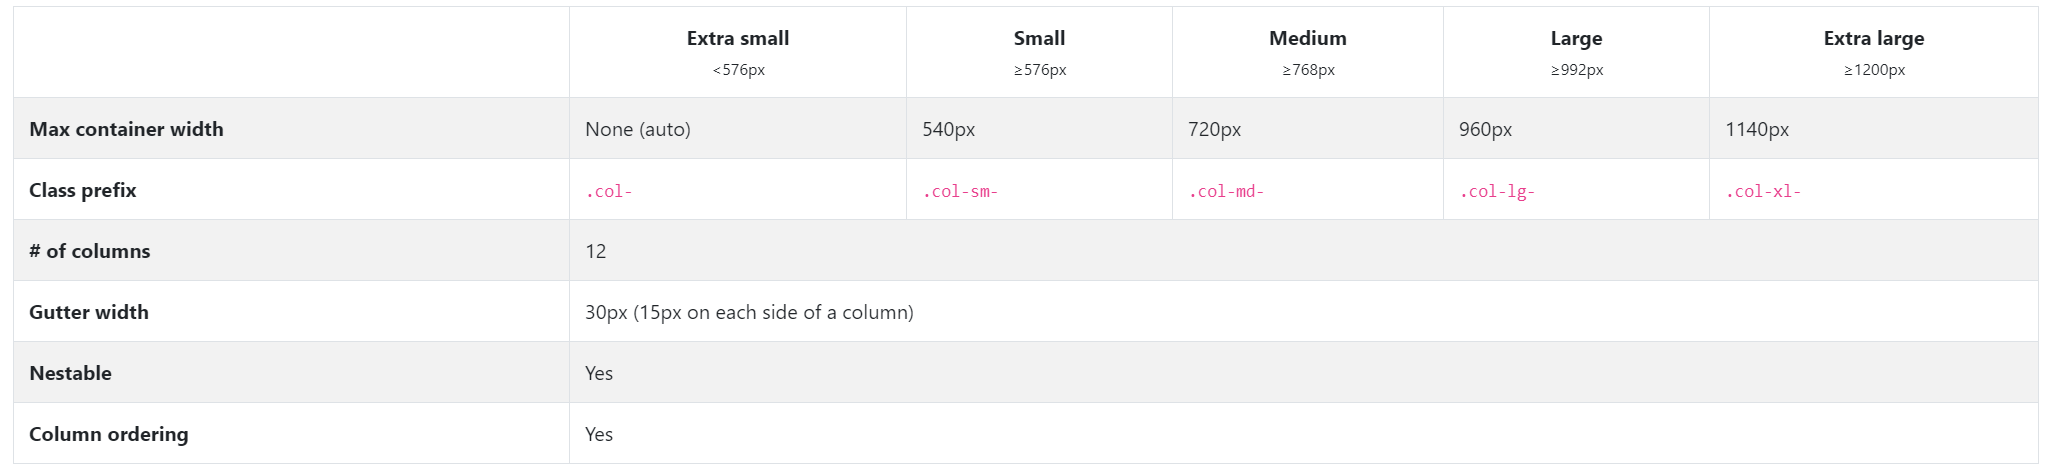
\includegraphics[scale=0.7]{gridoption_bootstrap.png}  
	\caption{Pilihan kelas grid pada Bootstrap} 
	\label{fig:choiceGridBootstrap}
\end{figure}

\subsection{Konten}
\subsubsection{Tabel}
\paragraph{Tabel Default}
Dengan penggunaan kelas \verb|.table| pada seluruh tag \texttt{<table>} maka \textit{style} pada bootstrap akan diterapkan, sehingga setiap tabel yang \textit{nested} akan diatur sesuai dengan \textit{parent} nya.
\begin{figure} [H]
	\centering  
	
\includegraphics[scale=0.7]{tablebasic_bootstrap.png}  
	\caption{Tabel default pada Bootstrap} 
	\label{fig:tableBootstrap}
\end{figure}

\begin{lstlisting}[language=HTML,  basicstyle=\ttfamily, frame=single, columns=fullflexible, keepspaces=true, breaklines=true, showstringspaces=false, label={lst:tableBootstrap}, caption=Tabel pada bootstrap 4] 
<table class="table">
<thead>
<tr>
<th scope="col">#</th>
<th scope="col">First</th>
<th scope="col">Last</th>
<th scope="col">Handle</th>
</tr>
</thead>
<tbody>
<tr>
<th scope="row">1</th>
<td>Mark</td>
<td>Otto</td>
<td>@mdo</td>
</tr>
<tr>
<th scope="row">2</th>
<td>Jacob</td>
<td>Thornton</td>
<td>@fat</td>
</tr>
<tr>
<th scope="row">3</th>
<td>Larry</td>
<td>the Bird</td>
<td>@twitter</td>
</tr>
</tbody>
</table>
\end{lstlisting}

\paragraph{Tabel dengan Garis Batas}
Penggunaan kelas \texttt{.table-bordered} akan membuat tabel memiliki garis batas untuk semua sisi didalam tabel dan \textit{cells}.

\begin{figure} [H]
	\centering  
	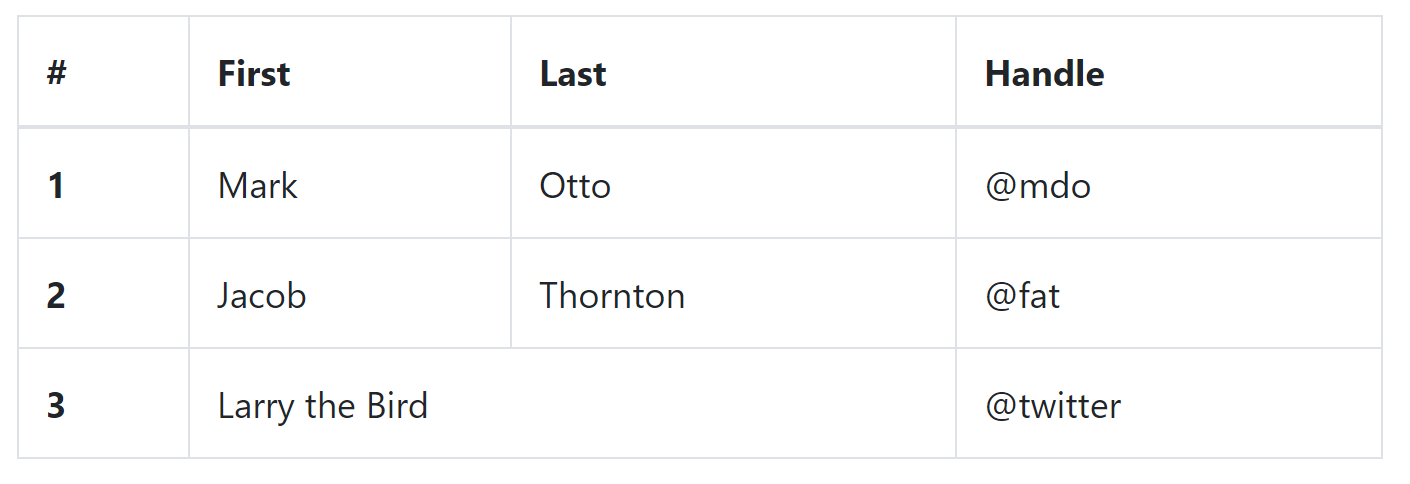
\includegraphics[scale=0.7]{tablebordered_bootstrap.png}  
	\caption{Tabel default pada Bootstrap} 
	\label{fig:tableBorderedBootstrap}
\end{figure}

\begin{lstlisting}[language=HTML,  basicstyle=\ttfamily, frame=single, columns=fullflexible, keepspaces=true, breaklines=true, showstringspaces=false, label={lst:tableborderedBootstrap}, caption=Kode tabel dengan garis batas pada bootstrap 4] 
<table class="table table-bordered">
<thead>
<tr>
<th scope="col">#</th>
<th scope="col">First</th>
<th scope="col">Last</th>
<th scope="col">Handle</th>
</tr>
</thead>
<tbody>
<tr>
<th scope="row">1</th>
<td>Mark</td>
<td>Otto</td>
<td>@mdo</td>
</tr>
<tr>
<th scope="row">2</th>
<td>Jacob</td>
<td>Thornton</td>
<td>@fat</td>
</tr>
<tr>
<th scope="row">3</th>
<td colspan="2">Larry the Bird</td>
<td>@twitter</td>
</tr>
</tbody>
</table>
\end{lstlisting}

\paragraph{Tabel dengan Warna Baris Berbeda}
Penggunaan kelas \texttt{.table-striped} akan membuat tabel memiliki warna baris berbeda batas antara baris genap dan ganjil didalam tag \texttt{<tbody>}.

\begin{figure} [H]
	\centering  
	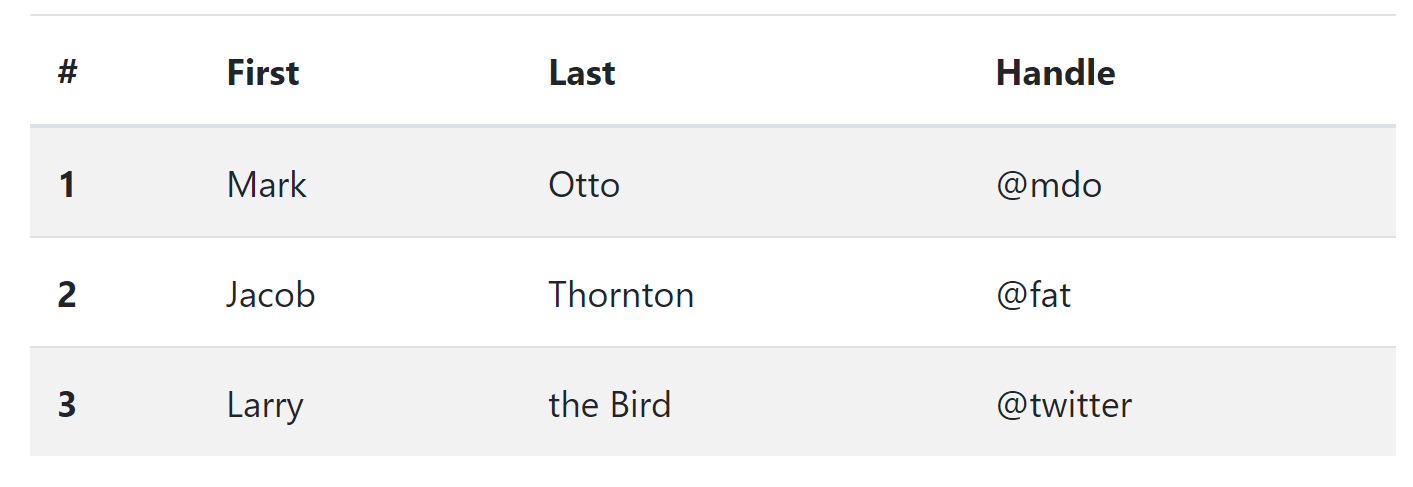
\includegraphics[scale=0.7]{tablestriped_bootstrap.png}  
	\caption{Tabel default pada Bootstrap} 
	\label{fig:tableStripedBootstrap}
\end{figure}

\begin{lstlisting}[language=HTML,  basicstyle=\ttfamily, frame=single, columns=fullflexible, keepspaces=true, breaklines=true, showstringspaces=false, label={lst:tablestripedBootstrap}, caption=Kode tabel dengan warna baris berbeda pada bootstrap 4.] 
<table class="table table-striped">
<thead>
<tr>
<th scope="col">#</th>
<th scope="col">First</th>
<th scope="col">Last</th>
<th scope="col">Handle</th>
</tr>
</thead>
<tbody>
<tr>
<th scope="row">1</th>
<td>Mark</td>
<td>Otto</td>
<td>@mdo</td>
</tr>
<tr>
<th scope="row">2</th>
<td>Jacob</td>
<td>Thornton</td>
<td>@fat</td>
</tr>
<tr>
<th scope="row">3</th>
<td colspan="2">Larry the Bird</td>
<td>@twitter</td>
</tr>
</tbody>
</table>
\end{lstlisting}


\subsubsection{Gambar}
Gambar dalam Bootstrap akan memiliki sifat \textit{responsive} dengan menerapkan kelas \texttt{.img-fluid} serta mengatur lebar gambar dengan properties \texttt{max-width: 100\%} dan \texttt{height: auto}. Sehingga gambar tidak pernah lebih besar dari \textit{parent} nya. 

\textit{Developer} dapat menyelaraskan (align) sebuah gambar ke kiri atau kanan dengan \texttt{helper float classes} atau \texttt{text alignment classes}. 
\begin{figure} [H]
	\centering  
	
\includegraphics[scale=0.7]{imgalign_bootstrap.PNG}  
	\caption{Menyelaraskan gambar ke kanan dan kiri pada bootstrap} 
	\label{fig:imageAlignStripedBootstrap}
\end{figure}
\begin{lstlisting}[language=HTML,  basicstyle=\ttfamily, frame=single, columns=fullflexible, keepspaces=true, breaklines=true, showstringspaces=false, label={lst:imgalignBootstrap}, caption=Image Align pada bootstrap 4.]
<img src="..." class="rounded float-left" alt="...">
<img src="..." class="rounded float-right" alt="...">
\end{lstlisting}



\subsection{Komponen}
\subsubsection{Formulir}
\textit{Form} pada Bootstrap menyediakan beragam tipe input sesuai dengan kebutuhan \textit{user}. Contohnya penggunaan kelas \texttt{email} untuk \textit{input} email atau \texttt{number} untuk input berupa angka.
\subsubsection{Form Controls}
\textit{Developer} dapat membuat form menggunakan kelas \texttt{.form-control}. Kelas ini terdiri dari beberapa tag seperti tag \texttt{<input>, <select>} dan \texttt{<textarea>}.
\begin{lstlisting}[language=HTML,  basicstyle=\ttfamily, frame=single, columns=fullflexible, keepspaces=true, breaklines=true, showstringspaces=false, label={lst:formControlsBootstrap}, caption=Form controls pada bootstrap 4.]  
<form>
<div class="form-group">
<label for="exampleFormControlInput1">Email address</label>
<input type="email" class="form-control" id="exampleFormControlInput1" placeholder="name@example.com">
</div>
<div class="form-group">
<label for="exampleFormControlSelect1">Example select</label>
<select class="form-control" id="exampleFormControlSelect1">
<option>1</option>
<option>2</option>
<option>3</option>
<option>4</option>
<option>5</option>
</select>
</div>
<div class="form-group">
<label for="exampleFormControlSelect2">Example multiple select</label>
<select multiple class="form-control" id="exampleFormControlSelect2">
<option>1</option>
<option>2</option>
<option>3</option>
<option>4</option>
<option>5</option>
</select>
</div>
<div class="form-group">
<label for="exampleFormControlTextarea1">Example textarea</label>
<textarea class="form-control" id="exampleFormControlTextarea1" rows="3"></textarea>
</div>
</form>
\end{lstlisting}

\begin{figure} [H]
	\centering  
	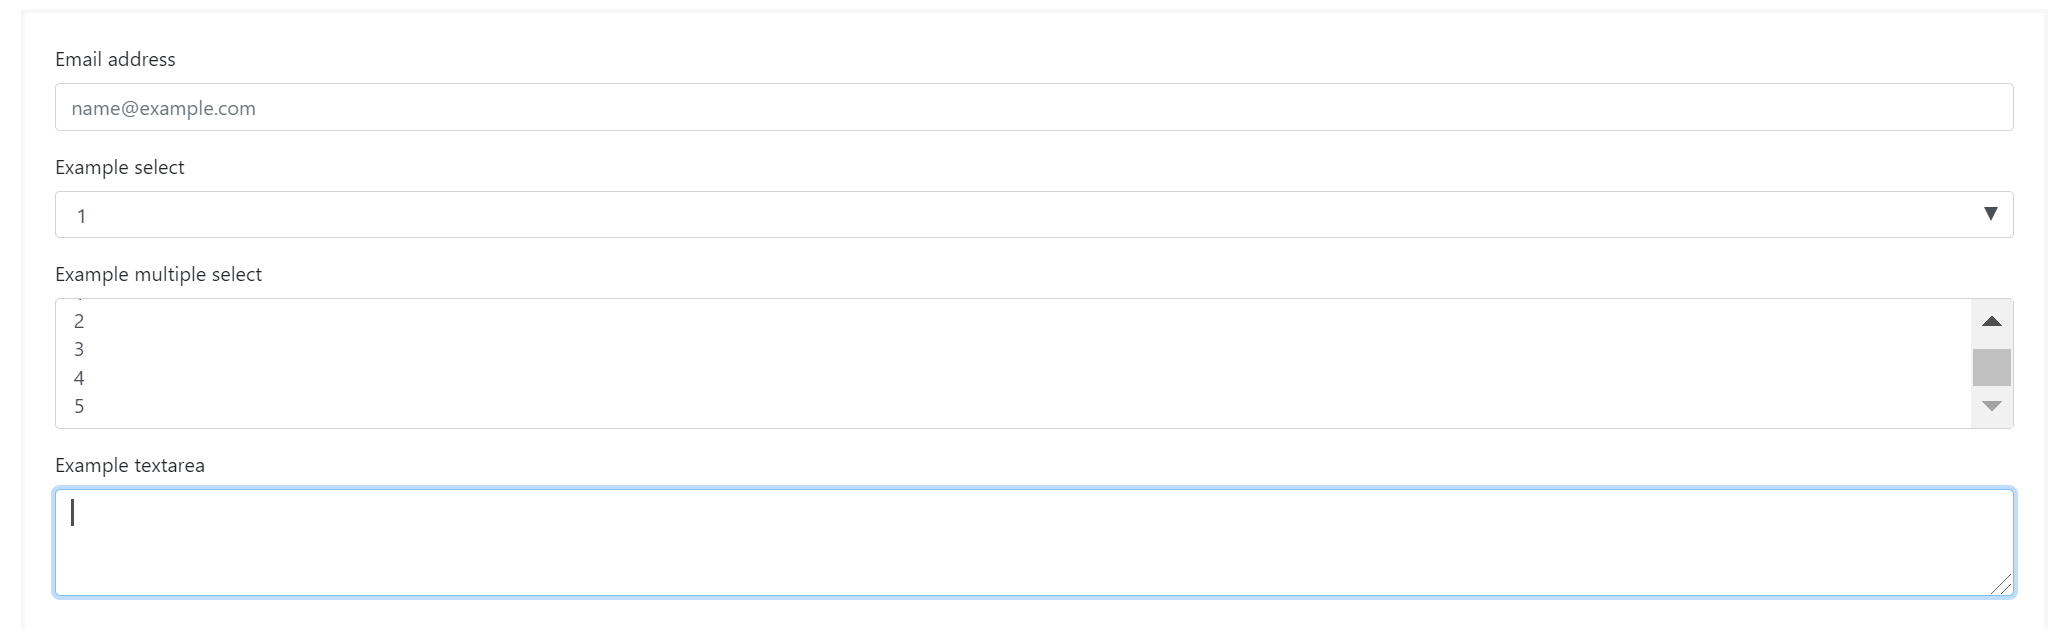
\includegraphics[scale=0.7]{formsbasic_bootstrap.png}  
	\caption{\textit{Forms Basic} pada Bootstrap} 
	\label{fig:formBootstrap}
\end{figure} 
\subsubsection{Column Sizing}
Bootstrap memungkinkan \textit{developer} untuk menempatkan sejumlah \texttt{.col} di dalam baris \texttt{.row} atau \texttt{.form} dengan lebar tertentu. Misalnya ada tiga buah kolom, kolom pertama memiliki lebar 7 dengan menggunakan kelas \texttt{.col-7} maka dua kolom sisanya akan memiliki lebar yang  memenuhi baris tersebut.
\begin{figure} [H]
	\centering  
	
\includegraphics[scale=0.7]{columnsizing_bootstrap.png}  
	\caption{\textit{Forms Basi}c pada Bootstrap} 
	\label{fig:columnSizingBootstrap}
\end{figure} 
\begin{lstlisting}[language=HTML,  basicstyle=\ttfamily, frame=single, columns=fullflexible, keepspaces=true, breaklines=true, showstringspaces=false, label={lst:columnsizingBootstrap}, caption=Column sizing pada bootstrap 4.] 
<form>
<div class="form-row">
<div class="col-7">
<input type="text" class="form-control" placeholder="City">
</div>
<div class="col">
<input type="text" class="form-control" placeholder="State">
</div>
<div class="col">
<input type="text" class="form-control" placeholder="Zip">
</div>
</div>
</form>
\end{lstlisting}
\subsubsection{Disabled Forms}
Penambahan atribut boolean \texttt{disabled} pada sebuah input membuat \textit{user} tidak bisa mengisi data pada \textit{field} tersebut. Untuk non-aktifkan seluruh \textit{field} pada sebuah kolom dapat menambahkan atribut \texttt{disabled} pada tag \texttt{<fieldset>}.
\begin{figure} [H]
	\centering  
	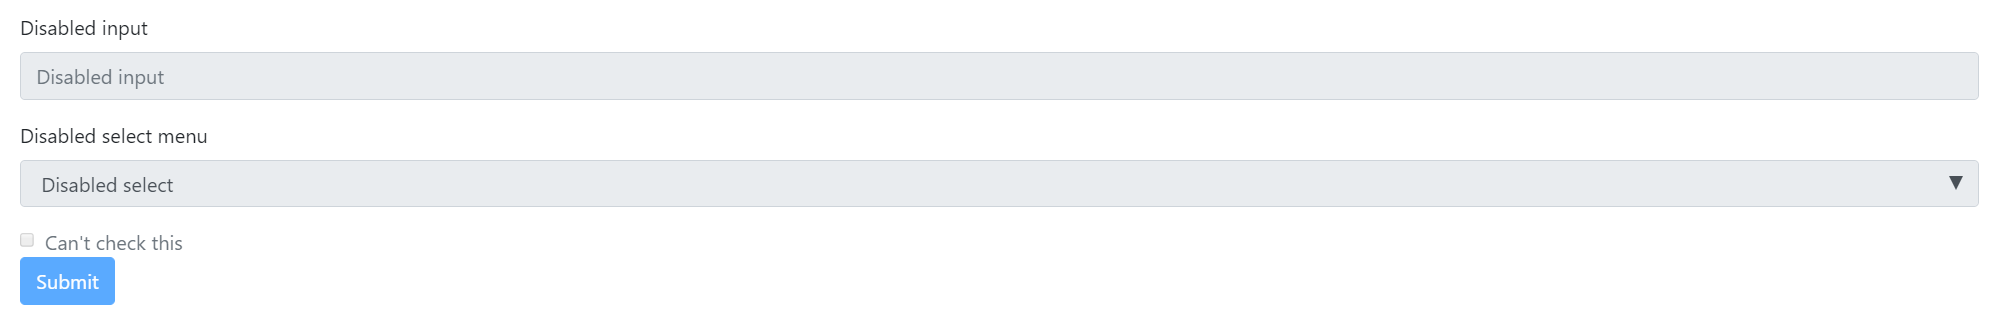
\includegraphics[scale=0.7]{disabledforms_bootstrap.png}  
	\caption{\textit{Disabled Basic} pada Bootstrap} 
	\label{fig:disabledFormBootstrap}
\end{figure}
\begin{lstlisting}[language=HTML,  basicstyle=\ttfamily, frame=single, columns=fullflexible, keepspaces=true, breaklines=true, showstringspaces=false, label={lst:disabledFormsBootstrap}, caption=Disabled forms pada bootstrap 4.]  
<form>
<fieldset disabled>
<div class="form-group">
<label for="disabledTextInput">Disabled input</label>
<input type="text" id="disabledTextInput" class="form-control"
placeholder="Disabled input">
</div>
<div class="form-group">
<label for="disabledSelect">Disabled select menu</label>
<select id="disabledSelect" class="form-control">
<option>Disabled select</option>
</select>
</div>
<div class="form-check">
<input class="form-check-input" type="checkbox" 
id="disabledFieldsetCheck" disabled>
<label class="form-check-label" for="disabledFieldsetCheck">
Can't check this
</label>
</div>
<button type="submit" class="btn btn-primary">Submit</button>
</fieldset>
</form>
\end{lstlisting}
\subsubsection{Button}
Bootstrap memasukan beberapa button dengan \textit{style} yang sudah didefinisikan sebelumnya, membuat setiap button akan memiliki makna nya sendiri.
\begin{figure} [H]
	\centering  
	
\includegraphics[scale=0.7]{buttons_bootstrap.png}  
	\caption{\textit{Button} pada Bootstrap} 
	\label{fig:buttonBootstrap}
\end{figure}
\begin{lstlisting}[language=HTML,  basicstyle=\ttfamily, frame=single, columns=fullflexible, keepspaces=true, breaklines=true, showstringspaces=false, label={lst:buttonBootstrap}, caption=Button pada bootstrap 4.] 
<button type="button" class="btn btn-primary">Primary</button>
<button type="button" class="btn btn-secondary">Secondary</button>
<button type="button" class="btn btn-success">Success</button>
<button type="button" class="btn btn-danger">Danger</button>
<button type="button" class="btn btn-warning">Warning</button>
<button type="button" class="btn btn-info">Info</button>
<button type="button" class="btn btn-light">Light</button>
<button type="button" class="btn btn-dark">Dark</button>

<button type="button" class="btn btn-link">Link</button>
\end{lstlisting}


\subsubsection{Button with Dropdowns}
\begin{lstlisting}[language=HTML,  basicstyle=\ttfamily, frame=single, columns=fullflexible, keepspaces=true, breaklines=true, showstringspaces=false, label={lst:buttonDropdownBootstrap}, caption=Button dropdown pada bootstrap 4.] 
<div class="input-group mb-3">
<div class="input-group-prepend">
<button class="btn btn-outline-secondary dropdown-toggle" type="button" data-toggle="dropdown"
aria-haspopup="true" aria-expanded="false">Dropdown</button>
<div class="dropdown-menu">
<a class="dropdown-item" href="#">Action</a>
<a class="dropdown-item" href="#">Another action</a>
<a class="dropdown-item" href="#">Something else here</a>
<div role="separator" class="dropdown-divider"></div>
<a class="dropdown-item" href="#">Separated link</a>
</div>
</div>
<input type="text" class="form-control" aria-label="Text input with dropdown button">
</div>

<div class="input-group">
<input type="text" class="form-control" aria-label="Text input with dropdown button">
<div class="input-group-append">
<button class="btn btn-outline-secondary dropdown-toggle" type="button" data-toggle="dropdown"
aria-haspopup="true" aria-expanded="false">Dropdown</button>
<div class="dropdown-menu">
<a class="dropdown-item" href="#">Action</a>
<a class="dropdown-item" href="#">Another action</a>
<a class="dropdown-item" href="#">Something else here</a>
<div role="separator" class="dropdown-divider"></div>
<a class="dropdown-item" href="#">Separated link</a>
</div>
</div>
</div>
\end{lstlisting}

\begin{figure} [H]
	\centering  
	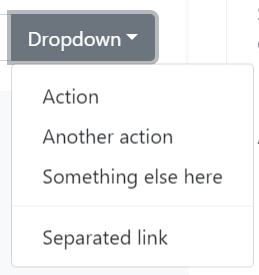
\includegraphics[scale=1.0]{buttonsdropdown_bootstrap.PNG}  
	\caption{Tombol \textit{dropdown} pada Bootstrap} 
	\label{fig:dropdownBootstrap}
\end{figure}

\subsubsection{Badge}
Kelas \texttt{badge} dan \texttt{.badge-*} di dalam sebuah \texttt{<a>} akan memberikan badge yang dapat diberi atribut \textit{hover} dan \textit{focus}. 
\begin{lstlisting}[language=HTML,  basicstyle=\ttfamily, frame=single, columns=fullflexible, keepspaces=true, breaklines=true, showstringspaces=false, label={lst:badgeBootstrap}, caption=Badge pada bootstrap 4.] 
<a href="#" class="badge badge-primary">Primary</a>
<a href="#" class="badge badge-secondary">Secondary</a>
<a href="#" class="badge badge-success">Success</a>
<a href="#" class="badge badge-danger">Danger</a>
<a href="#" class="badge badge-warning">Warning</a>
<a href="#" class="badge badge-info">Info</a>
<a href="#" class="badge badge-light">Light</a>
<a href="#" class="badge badge-dark">Dark</a>
\end{lstlisting}

\begin{figure} [H]
	\centering  
	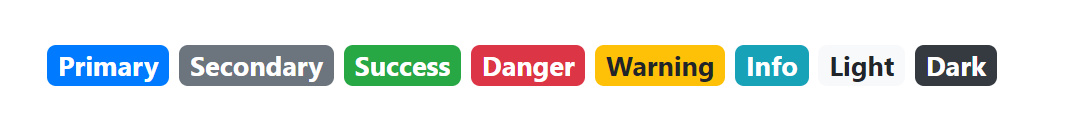
\includegraphics[scale=1.0]{badge_bootstrap.PNG}  
	\caption{Badge pada Bootstrap} 
	\label{fig:badgeBootstrap}
\end{figure}

\subsubsection{Card}
\texttt{Card} adalah kontainer konten yang fleksibel dan bisa diatur lebarnya. Sebuah card memiliki sebuah \textit{headers} dan \textit{footers}.

\begin{lstlisting}[language=HTML,  basicstyle=\ttfamily, frame=single, columns=fullflexible, keepspaces=true, breaklines=true, showstringspaces=false, label={lst:cardBootstrap}, caption=Card pada bootstrap 4.] 
<div class="card">
<div class="card-header">
Featured
</div>
<div class="card-body">
<h5 class="card-title">Special title treatment</h5>
<p class="card-text">With supporting text below as 
a natural lead-in to additional content.</p>
<a href="#" class="btn btn-primary"card>Go somewhere</a>
</div>
</div>
\end{lstlisting}

\begin{figure} [H]
	\centering  
	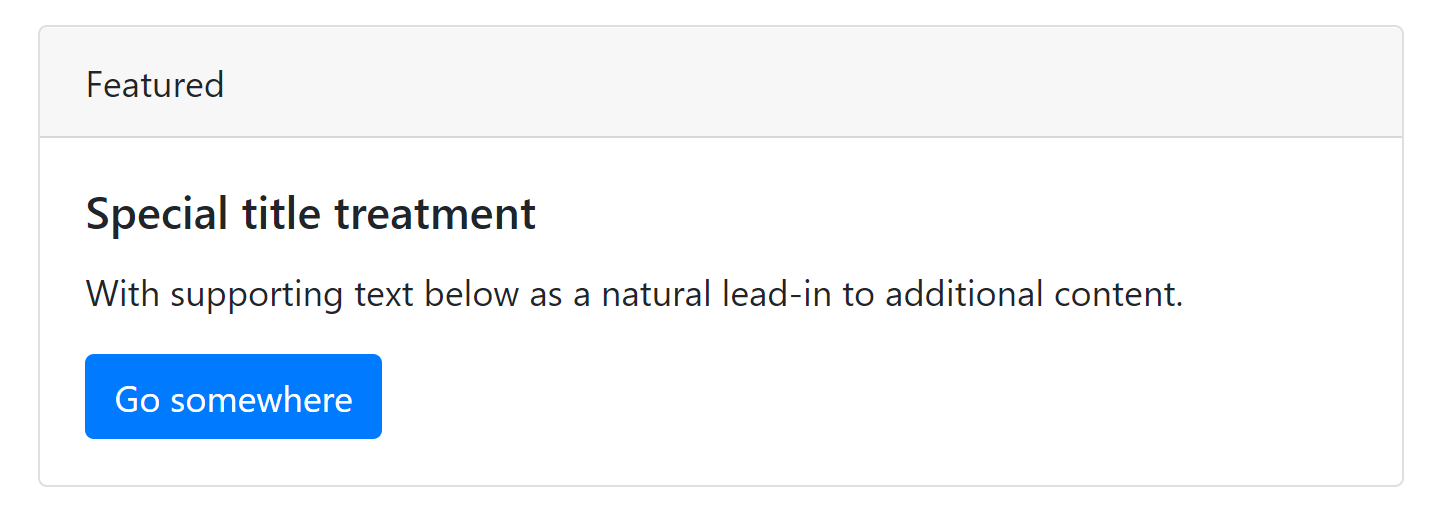
\includegraphics[scale=1.0]{card_bootstrap.PNG}  
	\caption{Card pada Bootstrap} 
	\label{fig:cardBootstrap}
\end{figure}

\subsubsection{Navigation Bar}
Navbar pada Bootstrap terdiri dari beberapa sub-komponen yang bisa digunakan sesuai dengan kebutuhan:
\begin{itemize}
	\item \texttt{.navbar-brand} : Komponen untuk menampilkan nama perusahaan, nama produk atau nama proyek.
	\item \texttt{.navbar-nav} : Komponen untuk membuat navigasi memiliki lebar yang memenuhi layar.
	\item \texttt{.navbar-toggler} : Komponen yang digunakan bersamaan dengan plugin untuk membuat efek jatuh dan perilaku navigasi lainnya.
	\item \texttt{.form-inline} : Komponen untuk pengaturan formulir dan aksi.
	\item \texttt{.collapse.navbar-collapse} : Komponen untuk mengelompokkan dan menyembunyikan \textit{navigation bar} dengan sebuah breakpoint induknya.
	%breakpoint : titik dimana terjadi perubahan (xs(br:0px), sm.. )
\end{itemize}
Berikut ini merupakan semua sub-komponen yang termasuk dalam navigation bar, navbar mengimplementasikan tema \texttt{light-themed} yang secara otomatis menyembunyilan menu pada breakpoint \texttt{lg}
\begin{figure} [H]
	\centering  
	
\includegraphics[scale=1.0]{navbar_bootstrap.PNG}  
	\caption{Navigation Bar pada Bootstrap} 
	\label{fig:navBarBootstrap}
\end{figure}

\begin{lstlisting}[language=HTML,  basicstyle=\ttfamily, frame=single, columns=fullflexible, keepspaces=true, breaklines=true, showstringspaces=false, label={lst:navBarBootstrap}, caption=Navigation bar pada bootstrap 4.]  
<nav class="navbar navbar-expand-lg navbar-light bg-light">
<a class="navbar-brand" href="#">Navbar</a>
<button class="navbar-toggler" type="button" data-toggle="collapse" data-target="#navbarSupportedContent" 
aria-controls="navbarSupportedContent" aria-expanded="false" aria-label="Toggle navigation">
<span class="navbar-toggler-icon"></span>
</button>

<div class="collapse navbar-collapse" id="navbarSupportedContent">
<ul class="navbar-nav mr-auto">
<li class="nav-item active">
<a class="nav-link" href="#">Home <span class="sr-only">(current)</span></a>
</li>
<li class="nav-item">
<a class="nav-link" href="#">Link</a>
</li>
<li class="nav-item dropdown">
<a class="nav-link dropdown-toggle" href="#" id="navbarDropdown" role="button" 
data-toggle="dropdown" aria-haspopup="true" aria-expanded="false">
Dropdown
</a>
<div class="dropdown-menu" aria-labelledby="navbarDropdown">
<a class="dropdown-item" href="#">Action</a>
<a class="dropdown-item" href="#">Another action</a>
<div class="dropdown-divider"></div>
<a class="dropdown-item" href="#">Something else here</a>
</div>
</li>
<li class="nav-item">
<a class="nav-link disabled" href="#">Disabled</a>
</li>
</ul>
<form class="form-inline my-2 my-lg-0">
<input class="form-control mr-sm-2" type="search" placeholder="Search" aria-label="Search">
<button class="btn btn-outline-success my-2 my-sm-0" type="submit">Search</button>
</form>
</div>
</nav>
\end{lstlisting}

\subsubsection{Modal}
Bagaimana Modal bekerja :
\begin{itemize}
	\item Modal dibangun dengan HTML, CSS dan Javascript. 
	\item Menekan modal "backdrop" otomatis menutup komponen modal.
	\item Bootstrap hanya mendukung satu modal dalam sebuah window pada satu waktu. Penggunaan modal yang bercabang dalam Bootstrap dipercaya memberikan \textit{user experience} yang buruk.
	\item Modal menggunakann \texttt{position: fixed} yang diletakkan pada posisi teratas dalam kode agar terhindar dari \textit{bug} yang disebabkan elemen lain yang memiliki posisi \textit{fixed}. 
\end{itemize}
Komponen modal terdiri dari modal headerm modal body dan modal footer (opsional).
\begin{figure} [H]
	\centering  
	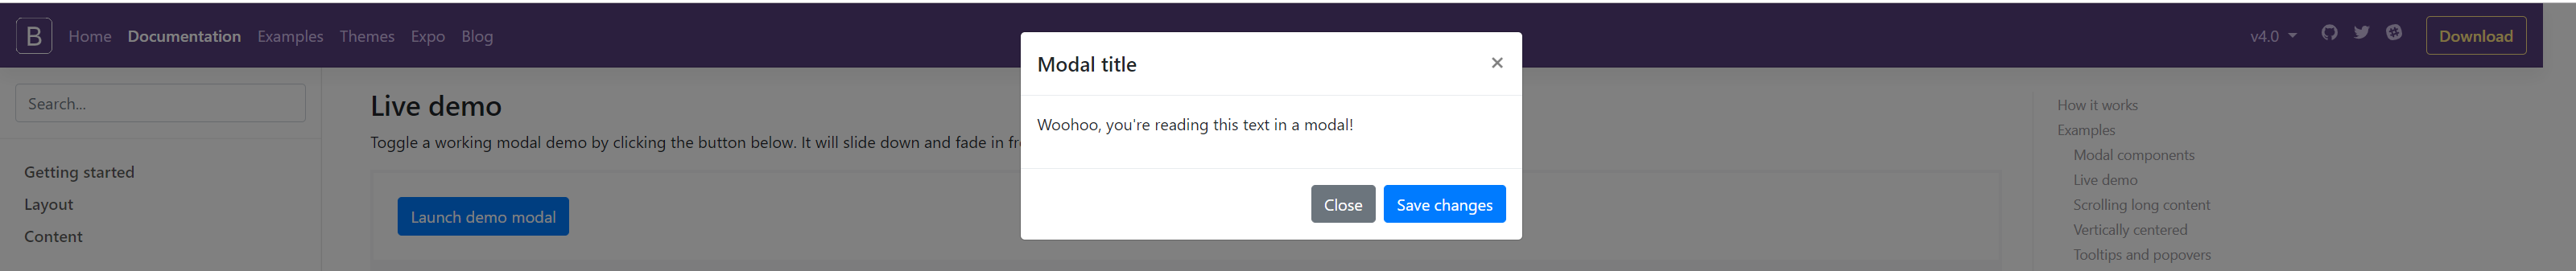
\includegraphics[scale=0.5]{livemodal_bootstrap.png}  
	\caption{Modal pada Bootstrap} 
	\label{fig:modalBootstrap}
\end{figure}

\begin{lstlisting}[language=HTML,  basicstyle=\ttfamily, frame=single, columns=fullflexible, keepspaces=true, breaklines=true, showstringspaces=false, label={lst:modalBootstrap}, caption=Modal bar pada bootstrap 4.] 
<!-- Button trigger modal -->
<button type="button" class="btn btn-primary" data-toggle="modal" data-target="#myModal">
Launch demo modal
</button>

<!-- Modal -->
<div class="modal fade" id="exampleModal" tabindex="-1" role="dialog" 
aria-labelledby="exampleModalLabel" aria-hidden="true">
<div class="modal-dialog" role="document">
<div class="modal-content">
<div class="modal-header">
<h5 class="modal-title" id="exampleModalLabel">Modal title</h5>
<button type="button" class="close" data-dismiss="modal" aria-label="Close">
<span aria-hidden="true">&times;</span>
</button>
</div>
<div class="modal-body">
...
</div>
<div class="modal-footer">
<button type="button" class="btn btn-secondary" data-dismiss="modal">Close</button>
<button type="button" class="btn btn-primary">Save changes</button>
</div>
</div>
</div>
</div>
\end{lstlisting}

\subsubsection{Ikon}
Bootstrap tidak memiliki \textit{library} ikon secara \textit{default}, sehingga ikon yang digunakan diambil dari \texttt{Font Awesome}. Penggunaan ikon dengan menggunakan tag \texttt{<i>} yang disertai dengan kelas \texttt{fa} (font-awesome). 

\begin{lstlisting}[language=HTML,  basicstyle=\ttfamily, frame=single, columns=fullflexible, keepspaces=true, breaklines=true, showstringspaces=false, label={lst:ikonBootstrap}, caption=Ikon pada bootstrap 4.]
<i class="fa fa-coffee"></i>
\end{lstlisting}

\begin{figure} [H]
	\centering  
	
\includegraphics[scale=1.0]{fa_coffee.PNG}  
	\caption{Ikon \textit{Coffee} pada Font Awesome} 
	\label{fig:fontAwesomeBootstrap}
\end{figure}
\subsubsection{Alert}
Alert menyediakan pesan umpan balik untuk user untuk berbagai tipe pesan peringatan yang tersedia. Untuk gaya yang sesuai \textit{developer} dapat menggunakan delapan kelas yang tersedia.
\begin{figure} [H]
	\centering  
	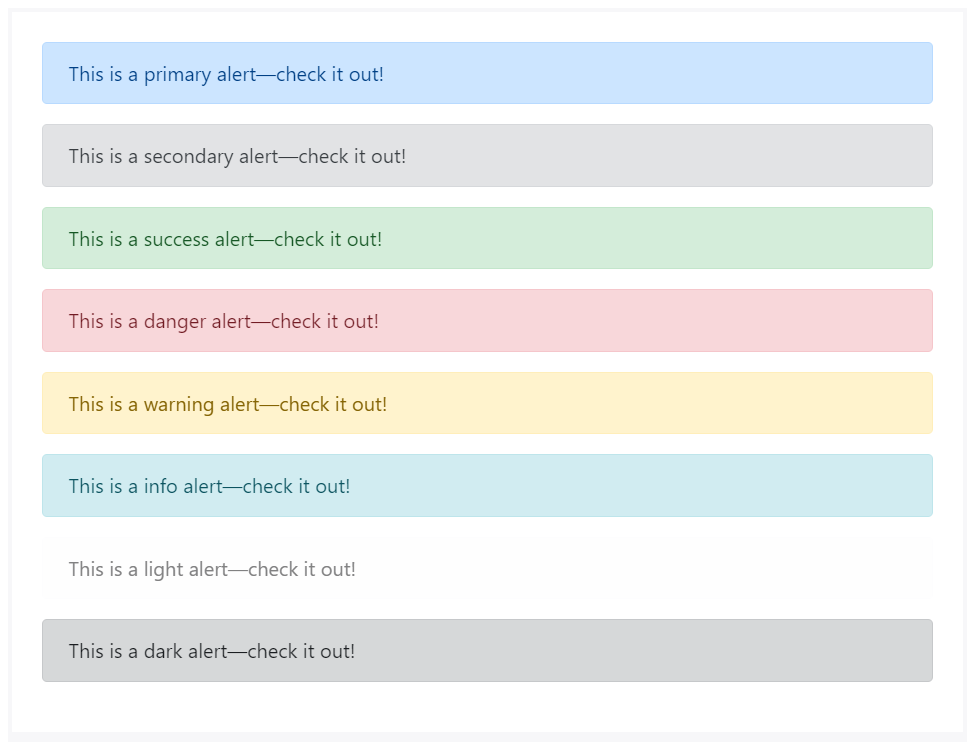
\includegraphics[scale=1.0]{alert_bootstrap.PNG}  
	\caption{Alert pada Bootstrap} 
	\label{fig:alertBootstrap}
\end{figure}
\begin{lstlisting}[language=HTML,  basicstyle=\ttfamily, frame=single, columns=fullflexible, keepspaces=true, breaklines=true, showstringspaces=false, label={lst:alertBootstrap}, caption=Alert pada bootstrap 4.] 
<div class="alert alert-primary" role="alert">
This is a primary alert—check it out!
</div>
<div class="alert alert-secondary" role="alert">
This is a secondary alert—check it out!
</div>
<div class="alert alert-success" role="alert">
This is a success alert—check it out!
</div>
<div class="alert alert-danger" role="alert">
This is a danger alert—check it out!
</div>
<div class="alert alert-warning" role="alert">
This is a warning alert—check it out!
</div>
<div class="alert alert-info" role="alert">
This is a info alert—check it out!
</div>
<div class="alert alert-light" role="alert">
This is a light alert—check it out!
</div>
<div class="alert alert-dark" role="alert">
This is a dark alert—check it out!
</div>
\end{lstlisting}

\section{DateTimePicker}
\texttt{DateTimePicker} dengan menggunakan jQuery untuk memilih tanggal dan waktu pada bagian forms. 
\subsubsection{Inline DateTimePicker}
Penggunaan plugin ini, memungkinkan \textit{users} untuk memilih tanggal dan waktu secara bersamaan.
\begin{figure} [H]
	\centering  
	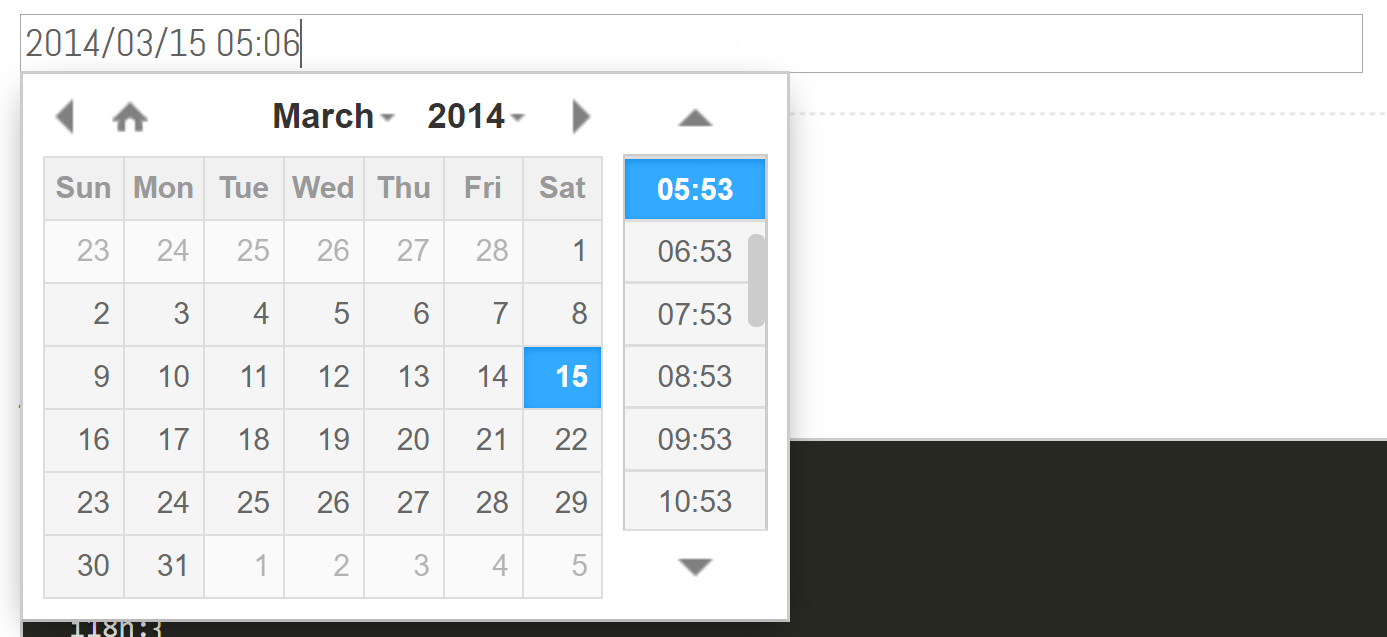
\includegraphics[scale=1.0]{datetimepicker_bootstrap4.PNG}  
	\caption{Datetimepicker pada Bootstrap} 
	\label{fig:datetimepickerBootstrap}
\end{figure}
\noindent 
Penggunaan nya dalam kode HTML sebagai berikut :
\begin{lstlisting}[language=HTML,  basicstyle=\ttfamily, frame=single, columns=fullflexible, keepspaces=true, breaklines=true, showstringspaces=false, label={lst:htmlPlugin}, caption=Kode HTML pada plugin.] 
<input id="datetimepicker" type="text" >
\end{lstlisting}

Penggunaan dalam kode Javascript sebagai berikut :

\begin{lstlisting}[language=HTML,  basicstyle=\ttfamily, frame=single, columns=fullflexible, keepspaces=true, breaklines=true, showstringspaces=false, label={lst:jQueryPlugin}, caption=Kode Inline DateTimePicker di jQuery.] 
%jQuery('#datetimepicker').datetimepicker();
\end{lstlisting}




